\documentclass[geye,green,kindle,cn]{elegantnote}

\usepackage{makecell}
\usepackage{tabularx}
\usepackage{graphicx}
\usepackage{listings}
\usepackage{xcolor}

\title{「ROS」学习笔记}
\author{\href{https://accelerator-blog.com}{陈策}}
\version{0.0}
\date{2019 年 11 月 21 日}
\begin{document}
\maketitle
\centerline{
\includegraphics[width=0.32\textwidth]{src/TsinghuaLogo.pdf}}

\begin{table}[htbp]
    \centering
    \caption{中文术语表A} \label{table:ChineseTermTableA}
    \begin{tabular}{p{80pt}<{\centering}p{80pt}<{\centering}}
    \Xhline{1.0pt}
    \textbf{英文术语} & 
    \textbf{中文术语} \\
    \hline
    Node &
    节点 \\
    Master &
    主节点 \\
    Package &
    功能包 \\
    Metapackage &
    元功能包 \\
    Dependent Package &
    依赖包 \\
    Message &
    消息 \\
    Service &
    服务 \\
    Topic &
    话题 \\
    Service Server &
    服务服务器 \\
    Service Client &
    服务客户端 \\
    Parameter Server &
    参数服务器 \\
    Publisher &
    发布者 \\
    Subscriber &
    订阅者 \\
    \Xhline{1.0pt}
    \end{tabular}
\end{table}

\begin{table}[htbp]
    \centering
    \caption{中文术语表B} \label{table:ChineseTermTableB}
    \begin{tabular}{p{80pt}<{\centering}p{80pt}<{\centering}}
    \Xhline{1.0pt}
    \textbf{英文术语} & 
    \textbf{中文术语} \\
    \hline
    Launch &
    启动 \\
    Client Library &
    客户端库 \\
    Repositories &
    存储库 \\
    Namespace &
    命名空间 \\
    Base Name &
    基本名称 \\
    Global Name &
    全局名称 \\
    Private Name &
    私有名称 \\
    Relative Name &
    相对名称 \\
    Node Handle &
    节点句柄 \\
    Timer &
    计时器 \\
    Transform &
    变换 \\
    Master PC &
    总机 \\
    Host PC &
    主机 \\
    Build &
    构建 \\
    \Xhline{1.0pt}
    \end{tabular}
\end{table}

\begin{table}[htbp]
    \centering
    \caption{中文术语表C} \label{table:ChineseTermTableC}
    \begin{tabular}{p{80pt}<{\centering}p{80pt}<{\centering}}
    \Xhline{1.0pt}
    \textbf{英文术语} & 
    \textbf{中文术语} \\
    \hline
    Motion Planning &
    运动规划 \\
    Odometry &
    侧位 \\
    Pose &
    姿态 \\
    Play/Replay &
    回放 \\
    Introspection &
    自检 \\
    Icon &
    图标 \\
    Dead Reckoning &
    导航推测 \\
    Base &
    基座 \\
    Link &
    连杆 \\
    Joint &
    关节 \\
    End Effector &
    末端执行器 \\
    \Xhline{1.0pt}
    \end{tabular}
\end{table}

\section{机器人软件平台}
\subsection{平台的组件}
\subsection{机器人软件平台}
\subsection{机器人软件平台的必要性}
\subsection{机器人软件平台将带来的未来}
\section{机器人操作系统 ROS}
\subsection{ROS 简介}
\subsection{元操作系统}
\subsection{ROS的目的}
\subsection{ROS的组件}
\subsection{ROS的生态系统}
\subsection{ROS的历史}
\subsection{ROS的版本}
\subsubsection{版本规则}
\subsubsection{版本周期}
\subsubsection{选择版本}
\section{搭建ROS开发环境}
\subsection{安装ROS}
\subsubsection{常规安装}
\subsubsection{简易安装}
\subsection{搭建ROS开发环境}
\subsubsection{ROS配置}
\subsubsection{集成开发环境(IDE)}
\subsection{ROS操作测试}
\section{ROS的重要概念}
\subsection{ROS术语}
\subsubsection{ROS}
ROS是一个用于开发机器人应用程序的、类似操作系统的机器人软件平台。
\subsubsection{主节点}
主节点(master)负责节点到节点的连接和消息通信,类似于名称服务器(Name Server)。

roscore是它的运行命令,当您运行主节点时,可以注册每个节点的名字,并根据需要获取信息。

没有主节点,就不能在节点之间建立访问和消息交流(如话题和服务)。

主节点使用XML远程过程调用(XMLRPC,XML-Remote Procedure Call)与节点进行通信。XMLRPC是一种基于HTTP的协议,主节点不与连接到主节点的节点保持连接。换句话说,节点只有在需要注册自己的信息或向其他节点发送请求信息时才能访问主节点并获取信息。通常情况下,不检查彼此的连接状态。

当启动ROS时,主节点将获取用户设置的ROS\_MASTER\_URI变量中列出的URI地址 和端口。除非另外设置,默认情况下,URI地址使用当前的本地IP,端口使用11311。

\subsubsection{节点}
节点(node)是指在ROS中运行的最小处理器单元,可以把它看作一个可执行程序。

在ROS中,建议为一个目的创建一个节点,建议设计时注重可重用性。

节点在运行的同时,向主节点注册节点的名称,并且还注册发布者(publisher)、 订阅者(subscriber)、服务服务器(service server)、服务客户端(service client)的名称,且注册消息形式、URI地址和端口。

基于这些信息,每个节点可以使用话题和服务与其他节点交换消息。

节点使用XMLRPC与主站进行通信,并使用TCP/IP通信系列的XMLRPC或TCPROS5进行节点之间的通信。节点之间的连接请求和响应使用XMLRPC,而消息通信使用TCPROS,因为它是节点和节点之间的直接通信,与主节点无关。

URI地址和端口则使用存储于运行当前节点的计算机上的名为ROS\_HOSTNAME的环境变量作为URI地址,并将端口设置为任意的固有值。
\subsubsection{功能包}
功能包(package)是构成ROS的基本单元,ROS应用程序是以功能包为单位开发的。

功能包包括至少一个以上的节点或拥有用于运行其他功能包的节点的配置文件。它还包含功能包所需的所有文件,如用于运行各种进程的ROS依赖库、数据集和配置文件等。
\subsubsection{元功能包}
元功能包(metapackage)是一个具有共同目的的功能包的集合。
\subsubsection{消息}
节点之间通过消息(message)来发送和接收数据。

消息是诸如integer、floating point和boolean等类型的变量。

用户还可以使用诸如消息里包括消息的简单数据结构或列举消息的消息数组的结构。

使用消息的通信方法包括TCPROS,UDPROS等,根据情况使用单向消息发送/接收方式的话题(topic)和双向消息请求(request)/响应 (response)方式的服务(service)。
\subsubsection{话题}
话题(topic)就是“故事”。在发布者(publisher)节点关于故事向主节点注册之后,它以消息形式发布关于该故事的广告。

希望接收该故事的订阅者(subscriber)节点获得在主节点中以这个话题注册的那个发布者节点的信息。基于这个信息,订阅者节点直接连接到发布者节点,用话题发送和接收消息。

\subsubsection{发布与发布者}
发布(publish)是指以与话题的内容对应的消息的形式发送数据。

为了执行发布,发布者(publisher)节点在主节点上注册自己的话题等多种信息,并向希望订阅的订阅者节点发送消息。

发布者在节点中声明自己是执行发布的个体。单个节点可以成为多个发布者。
\subsubsection{订阅与订阅者}
订阅是指以与话题内容对应的消息的形式接收数据。

为了执行订阅,订阅者节点在主节点上注册自己的话题等多种信息,并从主节点接收那些发布此节点要订阅的话题的发布者节点的信息。基于这个信息,订阅者节点直接联系发布者节点来接收消息。

订阅者在节点中声明自己执行订阅的个体。单个节点可以成为多个订阅者。

注意:发布和订阅概念中的话题是异步的,这是一种根据需要发送和接收数据的好方法。另外,由于它通过一次的连接,发送和接收连续的消息,所以它经常被用于必须连续发送消息的传感器数据。然而,在某些情况下,需要一种共同使用请求和响应的同步消息交换方案。因此,ROS提供叫做服务(service)的消息同步方法。服务分为响应请求的服务服务器和请求后接收响应的服务客户端。与话题不同,服务是一次性的消息通信。当服务的请求和响应完成时,两个节点的连接被断开。

\subsubsection{服务}
服务(service)消息通信是服务客户端(service client)与服务服务器(service server)之间的同步双向消息通信。其中服务客户端请求对应于特定目的任务的服务,而服务服务器则负责服务响应。
\subsubsection{服务服务器}
服务服务器(service server)是以请求作为输入,以响应作为输出的服务消息通信的服务器。

请求和响应都是消息,服务器收到服务请求后,执行指定的服务,并将结果下发给服务客户端。

服务服务器用于执行指定命令的节点。
\subsubsection{服务客户端}
服务客户端(service client)是以请求作为输出并以响应作为输入的服务消息通信的客户端。

请求和响应都是消息,并发送服务请求到服务服务器后接收其结果。

服务客户端用于传达给定命令并接收结果值的节点。
\subsubsection{动作}
动作(action)是在需要像服务那样的双向请求的情况下使用的消息通信方式,不同点是在处理请求之后需要很长的响应,并且需要中途反馈值。

动作文件也非常类似于服务,目标(goal)和结果(result)对应于请求和响应。此外,还添加了对应于中途的反馈(feedback)。它由一个设置动作目标(goal)的动作客户端(action client)和一个动作服务器(action server)组成,动作服务器根据目标执行动作,并发送反馈和结果。

动作客户端和动作服务器之间进行异步双向消息通信。
\subsubsection{动作服务器}
动作服务器(action server)以从动作客户端接收的目标作为输入并且以结果和反馈值作为输出的消息通信的服务器。

在接收到来自客户端的目标值后,负责执行实际的动作。
\subsubsection{动作客户端}
动作客户端(action client)是以目标作为输出并以从动作服务器接收待结果和反馈值作为输入的消息通信的客户端。

它将目标交付给动作服务器,收到结果和反馈,并给出下一个指示或取消目标。
\subsubsection{参数}
ROS中的参数(parameter)是指节点中使用的参数。可以把它想象成一个Windows程序中的*.ini配置文件。

这些参数是默认(default)设置的,可以根据需要从外部读取或写入。尤其是,它可以通过使用外部的写入功能实时更改设置值,因此非常有用。
\subsubsection{参数服务器}
参数服务器(parameter server)是指在功能包中使用参数时,注册各参数的服务器。

参数服务器也是主节点的一个功能。
\subsubsection{catkin}
catkin是指ROS的构建系统。

ROS的构建系统使用CMake(Cross Platform Make),并在功能包目录中的CMakeLists.txt文件中描述构建环境。

在ROS中,我们将CMake修改成专为ROS定制的catkin构建系统。

catkin构建系统让用户方便使用与ROS相关的构建、功能包管理以及功能包之间的依赖关系等。现在使用ROS的话,需要使用catkin而不是rosbuild。
\subsubsection{rosbuild}
ROS构建(rosbuild)是在构建catkin构建系统之前使用的构建系统,虽然仍有一些用户可以使用,但这只是为ROS版本兼容性保留的,并不是官方推荐的。

如果您必须使用rosbuild构建系统使用旧的功能包,我们建议您将rosbuild更改为catkin。
\subsubsection{roscore}
roscore是运行ROS主节点的命令,也可以在另一台位于同一个网络内的计算机上运行它,但除了支持多roscore的某些特殊情况,roscore在一个网络中只能运行一个。

运行ROS时,使用ROS\_MASTER\_URI变量中列出的URI地址和端口。

如果用户没有设置,会使用当前本地IP作为URI地址并使用端口11311。
\subsubsection{rosrun}
rosrun是ROS的基本运行命令,它用于在功能包中运行一个节点。

节点使用的URI地址将存储在当前运行节点的计算机上的ROS\_HOSTNAME环境变量作为URI地址,端口被设置为任意的固有值。
\subsubsection{roslaunch}
如果rosrun是执行一个节点的命令,那么roslaunch是运行多个节点的概念。

该命令允许运行多个确定的节点。其他功能还包括一些专为执行具有诸多选项的节点的ROS命令。roslaunch使用*.launch文件来设置可执行节点,它基于可扩展标记语言(XML),并提供XML标记形式的多种选项。
\subsubsection{bag}
用户可以保存ROS中发送和接收的消息的数据,这时用于保存的文件格式称为bag,是以*.bag作为扩展名。

在ROS中,这个功能包可以用来存储信息并在需要时可以回放以前的情况。

特别的,如果利用rosbag的记录和回放功能,在开发那些需要反复修改程序的算法的时候会非常有用。
\subsubsection{\href{http://wiki.ros.org/}{ROS Wiki}}
ROS的基本说明是一个基于wiki的页面,它解释了ROS提供的每个功能包和功能。
\subsubsection{存储库}
每一个公开的功能包在该功能包的wiki上指定一个存储库(repository)。

存储库是存储功能包的网站的URL地址,并使用源代码管理系统(如svn、hg和git)来管理问题、开发、下载等。许多当前可用的ROS功能包将github用作存储库。
\subsubsection{状态图}
上面描述的节点、话题、发布者和订阅者之间关系可以通过状态图(graph)直观地表示,它是当前正在运行的消息通信的图形表示,但不能为一次性服务创建状态图。

执行它是通过运行rqt\_graph功能包的rqt\_graph节点完成的。有两种执行命令:rqt\_graph和rosrun rqt\_graph rqt\_graph。
\subsubsection{名称}
节点、参数、话题和服务都有名称(name)。

当使用主节点的参数、话题和服务时,向主节点注册该名称并根据名称进行搜索,然后发送消息。

名称非常灵活,它们可以在运行时被更改,对于一个节点、参数、话题和服务,也能给其设定多个不同的名称。
\subsubsection{客户端库}
ROS是一个客户端库(client library),它为各种语言提供开发环境,以减少对所用语言的依赖性。主要的客户端库包括C++、Python和Lisp。其他语言包括Java、 Lua、.NET、EusLisp和R。
\subsubsection{URI}
统一资源标识符(URI,Uniform Resource Identifier)是代表Internet上资源的唯一地址。

该URI被用作Internet协议中的标识符,是在Internet上所需的基本条件。 
\subsubsection{MD5}
MD5(Message-Digest algorithm 5)是128位密码散列函数,它主要用于检查程序或文件的完整性,以查看它是否保持原样。

在使用ROS消息的通信中,使用MD5来检查消息发送/接收的完整性。
\subsubsection{RPC}
远程过程调用(RPC,Remote Procedure Call)意味着远程(Remote)计算机上的程序调用(Call)另一台计算机中的子程序(Procedure)。

这个利用TCP/IP、IPX等传输协议的技术在不需要程序员一一进行编程的情况下也能允许计算机在另一个地址空间通过远程控制运行函数或子程序。
subsubsection{XML}
可扩展标记语言(XML,Extensible Markup Language)是W3C推荐用于创建其他特殊用途标记语言的通用标记语言,它是通过使用标签来指定数据结构的语言之一。

在ROS中用于*.launch、*.urdf和package.xml等各个部分。
\subsubsection{XMLRPC}
XML-Remote Procedure Call(XMLRPC)是一种RPC协议,其编码形式采用XML编码格式,而传输方式采用既不保持连接状态、也不检查连接状态的请求和响应方式的HTTP协议。

XMLRPC是一个非常简单的约定,仅用于定义小数据类型或命令,所以它比较简单。有了这个特点,XMLRPC非常轻便,支持多种编程语言,因此非常适合支持各种硬件和语言的ROS。
\subsubsection{TCP/IP}
传输控制协议(TCP,Transmission Control Protocol)是一种传输控制协议,通常被称为TCP/IP。

从互联网协议层的角度来看,它基于IP(Internet Protocol)且使用传输控制协议TCP,以此保证数据传输,并按照发送顺序进行发送/接收。

TCPROS消息和服务中使用的基于TCP/IP的消息方式称为TCPROS,而UDPROS消息及服务中使用的基于UDP的消息方式称为UDPROS。

在ROS中,常用的是TCPROS。
\subsubsection{CMakeLists.txt}
ROS构建系统的catkin基本上使用了CMake,因此在功能包目录的CMakeLists.txt文件中描述着构建环境。
subsubsection{package.xml}
包含功能包信息的XML文件,描述功能包名称、作者、许可证和依赖包。
\subsection{消息通信}
ROS以节点的形式开发的,节点是根据其目的细分的可执行程序的最小单位,节点通过消息(message)与其他的节点交换数据。
\begin{figure}[htbp]
    \centering
    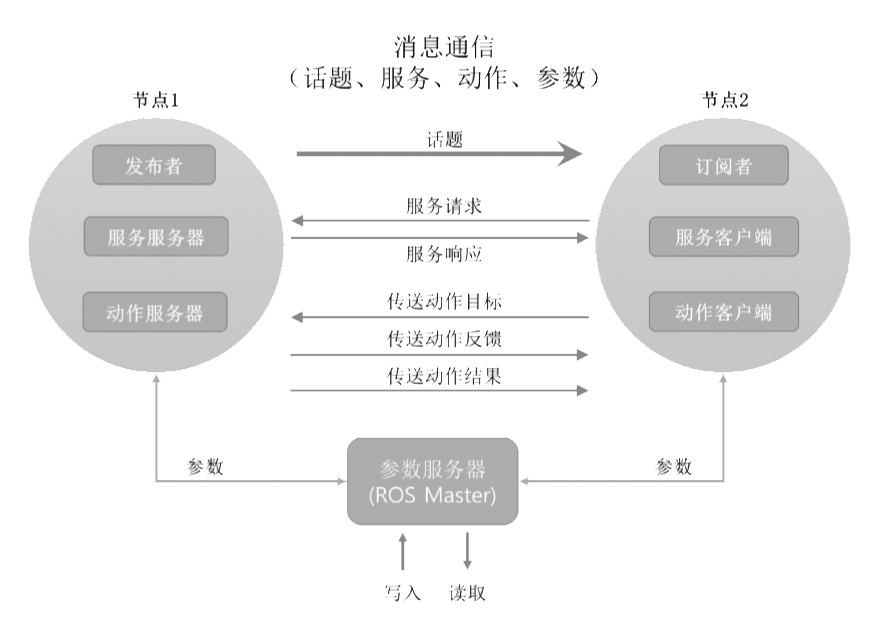
\includegraphics[width=1\linewidth]{src/A.png}
    \centering
    \caption{节点间的消息通信} \label{picture:A}
\end{figure}

这里的关键概念是节点之间的消息通信,它分为三种:单向消息发送/接收方式的话题(topic);双向消息请求/响应方式的服务 (service);双向消息目标(goal)/结果(result)/反馈(feedback)方式的动作(action)。
\begin{table}[htbp]
    \centering
    \begin{tabular}{p{200pt}}
    \Xhline{1.0pt}
    \textbf{种类,时序,方向,区别} \\
    \Xhline{1.0pt}
    话题,异步,单向,连续单向地发送/接收数据的情况 \\
    \hline
    服务,同步,双向,需要对请求给出即时响应的情况 \\
    \hline
    动作,异步,双向,请求与响应之间需要太长的时间,所以难以使用服务的情况,或需要中途反馈值的情况 \\
    \Xhline{1.0pt}
    \end{tabular}
    \centering
    \caption{话题、服务和动作之间的差异} \label{table:A}
\end{table}

节点中使用的参数可以从外部进行修改,这在大的框架中也可以被看作消息通信。
\subsubsection{话题(topic)}
话题消息通信是指发送信息的发布者和接收信息的订阅者以话题消息的形式发送和接收信息。

希望接收话题的订阅者节点接收的是与在主节点中注册的话题名称对应的发布者节点的信息。基于这个信息,订阅者节点直接连接到发布者节点来发送和接收消息。

话题是单向的,适用于需要连续发送消息的传感器数据,因为它们通过一次连接连续发送和接收消息。

单个发布者可以与多个订阅者进行通信,一个订阅者也可以在单个话题上与多个发布者进行通信。
\subsubsection{服务(service)}
服务消息通信是指请求服务的服务客户端与负责服务响应的服务服务器之间的同步双向服务消息通信。

前述的发布和订阅概念的话题通信方法是一种异步方法,是根据需要传输和接收给定数据的一种非常好的方法。然而,在某些情况下,需要一种同时使用请求和响应的同步消息交换方案。因此,ROS提供叫做服务的消息同步方法。

一个服务被分成服务服务器和服务客户端,其中服务服务器只在有请求(request)的时候才响应(response),而服务客户端会在发送请求后接收响应。

与话题不同,服务是一次性消息通信。因此,当服务的请求和响应完成时,两个连接的节点将被断开。

服务通常被用作请求机器人执行特定操作时使用的命令,或者用于根据特定条件需要产生事件的节点。由于它是一次性的通信方式,又因为它在网络上的负载很小,所以它也被用作代替话题的手段,是一种非常有用的通信手段。
\subsubsection{动作(action)}
动作消息通信是在如下情况使用的消息通信方式:服务器收到请求后直到响应所需的时间较长,且需要中途反馈值。

反馈在动作客户端(action client)和动作服务器(action server)之间执行异步双向消息通信,其中动作客户端设置动作目标(goal),而动作服务器根据目标执行指定的工作,并将动作反馈和动作结果发送给动作客户端。

与服务不同,动作通常用于指导复杂的机器人任务。在这种情况下,发布者、订阅者、服务服务器、服务客户端、动作服务器和动作客户端都存在于不同的节点中,这些节点需要连接才能进行消息通信。这时候,主节点帮助节点进行相互连接换,节点同时向主节点注册自己的信息,并从主节点获取其他节点希望通过主节点访问的节点的信息,然后,节点和节点直接连接进行消息通信。
\begin{figure}[htbp]
    \centering
    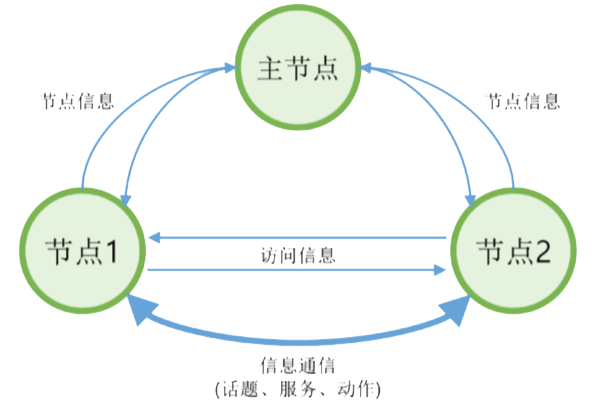
\includegraphics[width=1\linewidth]{src/B.png}
    \centering
    \caption{消息通信} \label{picture:B}
\end{figure}
\subsubsection{参数(parameter)}
信息通信主要分为话题、服务和动作,尽管参数严格的来说并不是消息通信,但从大的框架来看,参数也可以看作一种消息通信。

可以认为参数是节点中使用的全局变量。参数的用途与Windows程序中的*.ini配置文件非常类似。默认情况下,这些设置值是指定的,有需要时可以从外部读取或写入参数。特别是,由于可以通过使用来自外部的写入功能来实时地改变设置值,因此它是非常有用的,因为它可以灵活地应对多变的情况。
\subsubsection{消息通信的过程}
运行主节点:ROS主节点使用roscore命令来运行,并使用XMLRPC运行服务器。主节点为了节点与节点的连接,会注册节点的名称、话题、服务、动作名称、消息类型、URI地址和端口,并在有请求时将此信息通知给其他节点。
\begin{lstlisting}[frame=single,language=bash]
    $ roscore
\end{lstlisting}

运行订阅者节点:订阅者节点使用rosrun或roslaunch命令来运行。订阅者节点在运行时向主节点 注册其订阅者节点名称、话题名称、消息类型、URI地址和端口。主节点和节点使用 XMLRPC进行通信。
\begin{lstlisting}[frame=single,language=bash]
    $ rosrun PACKAGE_NAME NODE_NAME
    $ roslaunch PACKAGE_NAME LAUNCH_NAME
\end{lstlisting}

运行发布者节点:发布者节点(与订阅者节点类似)使用rosrun或roslaunch命令来运行。发布者节点向主节点注册发布者节点名称、话题名称、消息类型、URI地址和端口。主节点和节点使用XMLRPC进行通信。
\begin{lstlisting}[frame=single,language=bash]
    $ rosrun PACKAGE_NAME NODE_NAME
    $ roslaunch PACKAGE_NAME LAUNCH_NAME
\end{lstlisting}

通知发布者信息:主节点向订阅者节点发送此订阅者希望访问的发布者的名称、话题名称、消息类型、URI地址和端口等信息。主节点和节点使用XMLRPC进行通信。

订阅者节点的连接请求:订阅者节点根据从主节点接收的发布者信息,向发布者节点请求直接连接。在这种情况下,要发送的信息包括订阅者节点名称、话题名称和消息类型。发布者节点和订阅者节点使用XMLRPC进行通信。

发布者节点的连接响应:发布者节点将TCP服务器的URI地址和端口作为连接响应发送给订阅者节点。发布者节点和订阅者节点使用XMLRPC进行通信。

TCPROS连接:订阅者节点使用TCPROS创建一个与发布者节点对应的客户端,并直接与发布者节点连接。节点间通信使用一种称为TCPROS的TCP/IP方式。

发送消息:发布者节点向订阅者节点发送消息。节点间通信使用一种称为TCPROS的TCP/IP方式。

服务请求及响应:上述内容相当于消息通信中的话题。话题消息通信是只要发布者或订阅者不停止,会 持续地发布和订阅。服务分为两种:服务客户端(请求服务后等待响应)、服务服务器(收到服务请求后执行指定的任务,并发送响应),服务服务器和客户端之间的连接与上述发布者和订阅者之间的TCPROS连接相同,但是与话题不同,服务只连接一次,在执行请求和响应之后彼此断开连接。如果有必要,需要重新连接。

动作的目标、结果和反馈:动作(action)在执行的方式上好像是在服务(service)的请求(goal)和响应 (result)之间仅仅多了中途反馈环节,但实际的运作方式与话题相同。事实上,如果使用rostopic命令来查阅话题,那么可以看到该动作的goal、status、cancel、result和feedback等五个话题。动作服务器和客户端之间的连接与上述发布者和订阅中的TCPROS连接相同,但某些用法略有不同,动作客户端发送取消命令或服务器发送结果值会中断连接。
\subsection{消息}
消息(message)是用于节点之间的数据交换的一种数据形式。话题、服务和动作都使用消息。消息可以是简单的数据结构,或者是包含消息的简单的数据结构,也可以是消息数组结构。另外,ROS中常用的头(header、std\_msgs/Header)也可以作为消息来使用。这些消息由两种类型组成:字段类型(fieldtype)和字段名称(fieldname)。
\begin{lstlisting}[frame=single,language=bash]
    fieldtype1 fieldname1
    fieldtype2 fieldname2
    fieldtype3 fieldname3
\end{lstlisting}

字段类型应填入ROS数据类型,如下表所示。
\begin{table}[htbp]
\centering
\begin{tabular}{p{35pt}<{\centering}|p{55pt}<{\centering}|p{40pt}<{\centering}|p{40pt}<{\centering}} 
\Xhline{1.0pt}
\textbf{\small{ROS数据类型}} &
\textbf{\small{序列化(Serialization)}} &
\textbf{\small{C++数据类型}} &
\textbf{\small{Python数据类型}} \\
\Xhline{1.0pt}
\scriptsize{bool} &
\scriptsize{unsigned 8-bit int} &
\scriptsize{uint8\_t} &
\scriptsize{bool} \\
\hline
\scriptsize{int8} &
\scriptsize{signed 8-bit int} &
\scriptsize{int8\_t} &
\scriptsize{int} \\
\hline
\scriptsize{uint8} &
\scriptsize{unsigned 8-bit int} &
\scriptsize{uint8\_t} &
\scriptsize{int} \\
\Xhline{1.0pt}
\end{tabular}
\centering
\caption{数据类型A} \label{table:DatatypeA}
\end{table}

\begin{table}[htbp]
\centering
\begin{tabular}{p{35pt}<{\centering}|p{55pt}<{\centering}|p{40pt}<{\centering}|p{40pt}<{\centering}} 
\Xhline{1.0pt}
\textbf{\small{ROS数据类型}} &
\textbf{\small{序列化(Serialization)}} &
\textbf{\small{C++数据类型}} &
\textbf{\small{Python数据类型}} \\
\Xhline{1.0pt}
\scriptsize{int16} &
\scriptsize{signed 16-bit int} &
\scriptsize{int16\_t} &
\scriptsize{int} \\
\scriptsize{uint16} &
\scriptsize{unsigned 16-bit int} &
\scriptsize{uint16\_t} &
\scriptsize{int} \\
\hline
\scriptsize{int32} &
\scriptsize{signed 32-bit int} &
\scriptsize{int32\_t} &
\scriptsize{int} \\
\hline
\scriptsize{uint32} &
\scriptsize{unsigned 32-bit int} &
\scriptsize{uint32\_t} &
\scriptsize{int} \\
\hline
\scriptsize{int64} &
\scriptsize{signed 64-bit int} &
\scriptsize{int64\_t} &
\scriptsize{long} \\
\hline
\scriptsize{uint64} &
\scriptsize{unsigned 64-bit int} &
\scriptsize{uint64\_t} &
\scriptsize{long} \\
\hline
\scriptsize{float32} &
\scriptsize{32-bit IEEE float} &
\scriptsize{float} &
\scriptsize{float} \\
\hline
\scriptsize{float64} &
\scriptsize{64-bit IEEE float} &
\scriptsize{double} &
\scriptsize{float} \\
\hline
\scriptsize{string} &
\scriptsize{ascii string} &
\scriptsize{std::string} &
\scriptsize{str} \\
\hline
\scriptsize{time} &
\scriptsize{secs/nsecs unsigned 32-bit ints} &
\scriptsize{ros::Time} &
\scriptsize{rospy.Time} \\
\Xhline{1.0pt}
\end{tabular}
\centering
\caption{数据类型B} \label{table:DatatypeB}
\end{table}

\begin{table}[htbp]
\centering
\begin{tabular}{p{35pt}<{\centering}|p{55pt}<{\centering}|p{40pt}<{\centering}|p{40pt}<{\centering}} 
\Xhline{1.0pt}
\textbf{\small{ROS数据类型}} &
\textbf{\small{序列化(Serialization)}} &
\textbf{\small{C++数据类型}} &
\textbf{\small{Python数据类型}} \\
\Xhline{1.0pt}
\scriptsize{duration} &
\scriptsize{secs/nsecs signed 32-bit ints} &
\scriptsize{ros::Duration} &
\scriptsize{rospy.Duration} \\
\hline
\scriptsize{fixed-length} &
\scriptsize{no extra serialization} &
\scriptsize{boost::array, std::vector} &
\scriptsize{tuple} \\
\hline
\scriptsize{variable-length} &
\scriptsize{uint32 length prefix} &
\scriptsize{std::vector} &
\scriptsize{tuple} \\
\hline
\scriptsize{uint8[]} &
\scriptsize{uint32 length prefix} &
\scriptsize{std::vector} &
\scriptsize{bytes} \\
\hline
\scriptsize{bool[]} &
\scriptsize{uint32 length prefix} &
\scriptsize{std:: vector<uint8\_t>} &
\scriptsize{list of bool} \\
\Xhline{1.0pt}
\end{tabular}
\centering
\caption{数据类型C} \label{table:DatatypeC}
\end{table}

字段名称要填入指示数据的名称。

前面讲到ROS中常用的头(header、std\_ msgs/Header)可以作为消息来使用。更具体来说,正如std\_msgs32的Header.msg文件中描述,会记录序列号、时间戳和框架ID,利用它们在消息中记录消息的计数以及时间的计算。

std\_msgs/Header.msg
\begin{lstlisting}[frame=single,language=bash]
    # 序列号:是连续增加的ID,每个消息中依次递增+1。 
    uint32 seq 
    # 时间戳:具有两个子属性:以秒为单位的stamp.sec和以纳秒为单位的stamp.nsec。 
    time stamp 
    # 记录框架ID。 
    string frame_id
\end{lstlisting}
\subsubsection{Msg文件}
msg文件是用于话题的消息文件,扩展名为*.msg。
geometry\_msgs/Twist.msg
\begin{lstlisting}[frame=single,language=bash]
    Vector3  linear
    Vector3  angular
\end{lstlisting}
\subsubsection{Srv文件}
srv文件是服务使用的消息文件,扩展名为*.srv。与msg文件的主要区别在于三个连字符(---)作为分隔符,上层消息是服务请求消息,下层消息是服务响应消息。
sensor\_msgs/SetCameraInfo.srv
\begin{lstlisting}[frame=single,language=bash]
    sensor\_msgs/CameraInfo camera\_info 
    ---
    bool success 
    string status\_message
\end{lstlisting}
\subsubsection{Action文件}
action消息文件是动作中使用的消息文件,它使用*.action扩展名。与msg和srv不同,它不是一个比较常见的消息文件,所以没有典型的官方消息文件,但是可以像下面的例子一样使用它。与msg和srv文件的主要区别在于,三个连字符(---)在两个地方用作分隔符,第一部分是goal消息,第二部分是result消息,第三部分是feedback消息。
\begin{lstlisting}[frame=single,language=bash]
    geometry_msgs/PoseStamped start_pose 
    geometry_msgs/PoseStamped goal_pose 
    ---
    geometry_msgs/PoseStamped result_pose 
    ---
    float32 percent_complete 
\end{lstlisting}

最大的区别是来自action文件的feedback信息。action文件的goal消息和result消息与上述srv文件的请求消息和响应消息角色相同,但action文件的feedback消息用于传输指定进程执行过程中的中途值。

例子中,当机器人的出发点start\_pose和目标点 goal\_pose的位置和姿态作为请求值被传送时,机器人移动到预定的目标位置并且将发送最终到达的result\_pose的位置和姿态。另外,用percent\_complete消息,周期性地发送到达目标地点进程的百分比。 
\subsection{名称(name)}
ROS有一个称为图(graph)的抽象数据类型作为其基本概念。这显示了每个节点的连接关系以及通过箭头表达发送和接收消息(数据)的关系。为此,服务中使用的节点、话题、消息以及ROS中使用的参数都具有唯一的名称(name)。

话题名称分为相对的方法、全局方法和私有方法,用户可以在运行时更改节点的名称,而不需要运行额外的程序或更改源代码。方法包括命名空间(namespace)和重新映射(remapping)。
\subsection{坐标变换(TF)}
ROS中的坐标转换TF在描述组成机器人的每个部分、障碍物和外部物体时是最有用 的概念之一。这些可以被描述为位置(position)和方向(direction),统称为姿态 (pose)。在此,位置由x、y、z这3个矢量表示,而方向是用四元数(quaternion) x、y、z、w表示。四元数并不直观,因为它们没有使用我们在日常生活中使用的三元 数的角度表达方式:滚动角(roll)、俯仰角(pitch)和偏航角(yaw)。但这种四元 数方式不存在滚动、俯仰和偏航矢量的欧拉(Euler)方式具有的万向节死锁(gimbal lock)问题或速度问题,因此在机器人工程中人们更喜欢用四元数(quaternion)的形 式。因为同样的原因,ROS中也大量使用四元数 。当然,考虑到方便,它也提供将欧拉 值转换成四元数的功能。

类似上面说明的消息(message),TF使用以下格式。

geometry\_msgs/TransformStamped.msg
\begin{lstlisting}[frame=single,language=bash]
    Header header 
    string child_frame_id 
    Transform transform 
\end{lstlisting}

Header用于记录转换的时间,并使用名为child\_frame\_id的消息来表示下位的坐标。

为了表达坐标的转换值,使用以下数据形式描述对方的位置和方向:

transform.translation.x

transform.translation.y

transform.translation.z

transform.rotation.x

transform.rotation.y

transform.rotation.z

transform.rotation.w
\subsection{客户端库}
编程语言多如繁星。为了更快的性能和更好地控制硬件,会选择C++;为了更高的工作效率,会选择Python和Ruby。由于ROS需要支持具有多重目的特点的机器人,因此ROS提供面向多种语言的便利接口。具体来说,各个节点可以用各自的语言来编写,而节点间通过消息通信交换信息。其中,允许用各自的语言编写的软件模块就是客户端库(client library)。常用且具有代表性的库有支持C++的roscpp、支持Python的rospy。
\subsection{异构设备间的通信}
ROS基本上支持异构设备间的通信。节点间的通信不受各节点所在的ROS底层的操作系统的种类的影响,也不受编程语言的影响,因此可以很容易地进行通信。
\subsection{文件系统}
\subsubsection{文件组织结构}
在ROS中,组成软件的基本单位是功能包(package),因此ROS应用程序是以功能包为单位开发的。功能包包含一个以上的节点(node,ROS中最小的执行处理器)或包含用于运行其他节点的配置文件。这些功能包也会以元功能包(metapackage)的形式来统一管理。元功能包是具有共同目的的功能包的集合体。每个功能包都包含一个名为package.xml的文件,该文件是一个包含功能包信息的XML文件,包括其名称,作者,许可证和依赖包。此外,ROS构建系统catkin基本上使用CMake,并在功能包目录中的CMakeLists.txt文件中描述构建环境。另外,它由节点的源代码和消息文件组成,用于节点之间的消息通信。

ROS的文件系统分为安装目录和用户工作目录。

安装ROS desktop版本后,在/opt目录中会自动生成名为ros的安装目录,里面会安装有roscore、rqt、RViz、机器人相关库、仿真和导航等核心实用程序。用户很少需要修改这个区域的文件。如果要修改以二进制文件形式分发的功能包,请找到包含源代码的功能包存储库之后利用在“~/catkin\_ws/src”目录下用“git clone [存储库地址]”命令直接复制源代码,而不是用“sudo apt-get install ros-kinetic-xxx”形式的功能包安装命令。

用户的工作目录可以在用户想要的位置创建,下面我们就使用Linux用户目录“~/catkin\_ws/(在Linux中,‘~/’指‘/home/用户名/’目录)”。

ROS功能包的安装方式有二进制文件安装和源代码安装两种。二进制文件安装是使用二进制形式的文 件,无需额外的构建,而源代码安装是下载该功能包的源代码之后由用户进行构建之后使用的方式。 根据功能包使用的目的不同选择不同的方式。如果需要修改安装包或者要检查源代码的内容,可以使 用后一种安装方法。下面用turtlebot3功能包的例子,介绍两种安装方法的不同之处。

1. 二进制文件安装
\begin{lstlisting}[frame=single,language=bash]
    $ sudo apt-get install ros-kinetic-turtlebot3
\end{lstlisting}

2. 源代码安装
\begin{lstlisting}[frame=single,language=bash]
    $ cd ~/catkin_ws/src
    $ git clone https://github.com/ROBOTIS-GIT/turtlebot3.git
    $ cd ~/catkin_ws/
    $ catkin_make
\end{lstlisting}
\subsubsection{安装目录}
ROS安装在“/opt/ros/[版本名称]”目录中。

“/opt/ros/kinetic”目录下包含bin、etc、include、lib、share目 录和一些配置文件。

ROS目录包含用户在安装ROS时选择的功能包和ROS运行程序。详情如下:

/bin  可执行的二进制文件

/etc   与ROS和catkin相关的配置文件

/include  头文件

/lib   库文件

/share  ROS功能包

env.*  配置文件

setup.*  配置文件
\subsubsection{工作目录}
用户可以在任意位置创建工作目录,但是为了方便,本书中将Linux用户目录“~/ catkin\_ws/”用作工作目录。也就是说,您将使用“/home/用户名/catkin\_ws”目录。

catkin\_ws的目录,由目录 build、devel和src组成。请注意,build和devel目录是在catkin\_make之后创建的。

工作目录是对用户创建的功能包和其他开发人员公开的功能包进行存储和构建的空间。用户在该目录中执行与ROS有关的大部分操作。详情如下:

/build  构建相关的文件

/devel  msg、srv头文件、用户包库、可执行文件

/src   用户功能包

目录“~/catkin\_ws/src”是用户源代码的空间。在这个目录中,用户可以保存和建立自己的ROS功能包或其他开发者开发的功能包。

下面列举了通常使用的目录和文件,但其文件组成会根据功能包的用途而有所不同:

/include  头文件

/launch  用于roslaunch的启动文件

/node  用于rospy的脚本

/msg  消息文件

/src   源代码文件

/srv   服务文件

CMakeLists.txt  构建配置文件

package.xml   功能包配置文件
\subsection{构建系统}
ROS的构建系统默认使用CMake(Cross Platform Make),其构建环境在功能包目录中的CMakeLists.txt文件中描述。在ROS中,CMake被修改为适合于ROS的“catkin”构建系统。在ROS中使用CMake的是为了在多个平台上构建ROS功能包。因为不同于只支持Unix系列的Make,CMake支持Unix类的Linux、BSD和OS X以外,还支持Windows系列。并且,它还支持Microsoft Visual Studio,也还可以轻松应用于Qt开发。此外,catkin构建系统可以轻松使用与ROS相关的构建、功能包管理和功能包之间的依赖关系。 
\subsubsection{创建功能包}
创建ROS功能包的命令如下。
\begin{lstlisting}[frame=single,language=bash]
    $ catkin_create_pkg [功能包名称] [依赖功能包1] [依赖功能包n] 
\end{lstlisting}

“catkin\_create\_pkg”命令在创建用户功能包时会生成catkin构建系统所需的CMakeLists.txt和package.xml文件的包目录。

ROS中的功能包名称全部是小写字母,不能包含空格。格式规则是将每个单词用下划线(\_)而不是短划线(-)连接起来。
\subsubsection{修改功能包配置文件(package.xml)}
必要的ROS配置文件之一的package.xml是一个包含功能包信息的XML文件,包括 功能包名称、作者、许可证和依赖功能包。

下面是对每个语句的说明:

<?xml>   这是一个定义文档语法的语句,随后的内容表明在遵循xml版本1.0。

<package>   从这个语句到最后</package>的部分是ROS功能包的配置部分。 

<name>    功能包的名称。使用创建功能包时输入的功能包名称。正如其他选项,用户可以随时更改。

<version>   功能包的版本。可以自由指定。

<description>  功能包的简要说明。通常用两到三句话描述。

<maintainer>  提供功能包管理者的姓名和电子邮件地址。

<license>   记录版权许可证。写BSD、MIT、Apache、GPLv3或LGPLv3即可。

<url>    记录描述功能包的说明,如网页、错误管理、存储库的地址等。根据功能包的类型,用户可以填写网站、错误跟踪(bugtracker)或存储库的地址。

<author>    记录参与功能包开发的开发人员的姓名和电子邮件地址。如果涉及多位开发人员,只需在下一行添加<author>标签。

<buildtool\_depend>  描述构建系统的依赖关系。我们正在使用catkin构建系统,因此输入catkin。

<build\_depend> 在编写功能包时写下您所依赖的功能包的名称。

<run\_depend> 填写运行功能包时依赖的功能包的名称。

<test\_depend> 填写测试功能包时依赖的功能包名称。

<export>    在使用ROS中未指定的标签名称时会用到<export>。最广泛使用的情况是元功能包的情况,这时用<export> <metapackage/> </export>格式表明是元功能包。

<metapackage>  在export标签中使用的官方标签声明,当前功能包为一个元功能包时声明它。

以下为一个Demo:
\begin{lstlisting}[frame=single,language=xml]
    <?xml version="1.0"?>
    <package> 
    <name>my_first_ros_pkg</name>
    <version>0.0.1</version>
    <description>The my_first_ros_pkg package</description>
    <license>Apache License 2.0</license>
    <author email="pyo@robotis.com">Yoonseok Pyo</author>
    <maintainer email="pyo@robotis.com">Yoonseok Pyo</maintainer>
    <url type="bugtracker">https://github.com/ROBOTIS-GIT/ros_turtorials/issues</url>
    <url type="repository">https://github.com/ROBOTIS-GIT/ros_turtorials.git</url>
    <url type="website">http://www.robotis.com</url>
    <buildtool_depend>catkin</buildtool_depend>
    <build_depend>std_msgs</build_depend>
    <build_depend>roscpp</build_depend>
    <run_depend>std_msgs</run_depend>
    <run_depend>roscpp</run_depend>
    <export></export>
    </package>
\end{lstlisting}
\subsubsection{修改构建配置文件(CMakelists.txt)}
ROS的构建系统catkin基本上使用CMake,并在功能包目录中的CMakeLists.txt文件中描述构建环境。在这个文件中设置可执行文件的创建、依赖包优先构建、连接器(linker)的创建等等。

构建配置文件(CMakeLists.txt)中的每一项如下所示。

第一条是操作系统中安装的cmake的最低版本。由于它目前被指定为版本2.8.3,所以如果使用低于此版本的cmake,则必须更新版本。
\begin{lstlisting}[frame=single,language=bash]
    cmake_minimum_required(VERSION 2.8.3) 
\end{lstlisting} 

project项是功能包的名称。只需使用用户在package.xml中输入的功能包名即可。请注意,如果功能包名称与package.xml中的<name>标记中描述的功能包名称不同,则在构建时会发生错误,因此需要注意。
\begin{lstlisting}[frame=single,language=bash]
    project(my_first_ros_pkg) 
\end{lstlisting}

find\_package项是进行构建所需的组件包。目前,roscpp和std\_msgs被添加为依赖包。如果此处没有输入功能包名称,则在构建时会向用户报错。换句话说,这是让用户先创建依赖包的选项。 
\begin{lstlisting}[frame=single,language=]
    find_package(catkin REQUIRED COMPONENTS  
     roscpp  
     std_msgs 
    )
\end{lstlisting}

以下是使用ROS以外的功能包时使用的方法。例如,使用Boost时,必须安装system功能包。功能如前面的说明,是让用户先创建依赖功能包的选项。
\begin{lstlisting}[frame=single,language=]
    find_package(Boost REQUIRED COMPONENTS system)
\end{lstlisting}

catkin\_python\_setup()选项是在使用Python,也就是使用rospy时的配置选项。其功能是调用Python安装过程setup.py。
\begin{lstlisting}[frame=single,language=]
    catkin_python_setup() 
\end{lstlisting}

add\_message\_files是添加消息文件的选项。FILES将引用当前功能包目录的msg目录中的*.msg文件,自动生成一个头文件(*.h)。在这个例子中,我们将使用消息文件Message1.msg和Message2.msg。
\begin{lstlisting}[frame=single,language=]
    add_message_files(
     FILES
     Message1.msg
     Message2.msg
    ) 
\end{lstlisting}

add\_service\_files是添加要使用的服务文件的选项。使用FILES会引用功能包目录中的srv目录中的*.srv文件。在这个例子中,用户可以选择使用服务文件Service1.srv和Service2.srv。
\begin{lstlisting}[frame=single,language=]
    add_service_files(
     FILES
     Service1.srv
     Service2.srv
    ) 
\end{lstlisting}

generate\_messages是设置依赖的消息的选项。此示例是将DEPENDENCIES选项设 置为使用std\_msgs消息包。 
\begin{lstlisting}[frame=single,language=]
    generate_messages(
     DEPENDENCIES  
     std_msgs 
    ) 
\end{lstlisting}

generate\_dynamic\_reconfigure\_options是使用dynamic\_reconfigure时加载要引用的配置文件的设置。
\begin{lstlisting}[frame=single,language=]
    generate_dynamic_reconfigure_options(
     cfg/DynReconf1.cfg
     cfg/DynReconf2.cfg
    ) 
\end{lstlisting}

以下是catkin构建选项。INCLUDE\_DIRS表示将使用INCLUDE\_DIRS后面的内部目录include的头文件。LIBRARIES表示将使用随后而来的功能包的库。CATKIN\_DEPENDS后面指定如roscpp或std\_msgs等依赖包。目前的设置是表示依赖于roscpp和std\_msgs。DEPENDS是一个描述系统依赖包的设置。
\begin{lstlisting}[frame=single,language=]
    catkin_package(
     INCLUDE_DIRS include
     LIBRARIES my_first_ros_pkg
     CATKIN_DEPENDS roscpp std_msgs
     DEPENDS system_lib
    )
\end{lstlisting}

include\_directories是可以指定包含目录的选项。目前设定为\${catkin\_INCLUDE\_DIRS},这意味着将引用每个功能包中的include目录中的头文件。当用户想指定一个额外的include目录时,写在\${catkin\_INCLUDE\_DIRS}的下一行即可。 
\begin{lstlisting}[frame=single,language=]
    include_directories(
     ${catkin_INCLUDE_DIRS}
    ) 
\end{lstlisting}

add\_library声明构建之后需要创建的库。以下是引用位于my\_first\_ros\_pkg功能包的src目录中的my\_first\_ros\_pkg.cpp文件来创建my\_first\_ros\_pkg库的命令。
\begin{lstlisting}[frame=single,language=]
    add_library(my_first_ros_pkg
     src/${PROJECT_NAME}/my_first_ros_pkg.cpp
    ) 
\end{lstlisting}

add\_dependencies是在构建该库和可执行文件之前,如果有需要预先生成的有依赖性的消息或dynamic\_reconfigure,则要先执行。以下内容是优先生成my\_first\_ros\_ pkg库依赖的消息及dynamic reconfigure的设置。
\begin{lstlisting}[frame=single,language=]
    add_dependencies(my_first_ros_pkg ${${PROJECT_NAME}_EXPORTED_TARGETS} ${catkin_EXPORTED_TARGETS})
\end{lstlisting}

add\_executable是对于构建之后要创建的可执行文件的选项。以下内容是引用src/my\_first\_ros\_pkg\_node.cpp文件生成my\_first\_ros\_pkg\_node可执行文件。如果有多个要引用的*.cpp文件,将其写入my\_first\_ros\_pkg\_node.cpp之后。如果要创建两个以上的可执行文件,需追加add\_executable项目。
\begin{lstlisting}[frame=single,language=]
    add_executable(my_first_ros_pkg_node src/my_first_ros_pkg_node.cpp)
\end{lstlisting}

如前面描述的add\_dependencies一样,add\_dependencies是一个首选项,是在构建库和可执行文件之前创建依赖消息和dynamic reconfigure的设置。下面介绍名为my\_first\_ros\_pkg\_node的可执行文件的依赖关系,而不是上面提到的库。在建立可执行文件之前,先创建消息文件的情况下会经常用到。
\begin{lstlisting}[frame=single,language=]
    add_dependencies(my_first_ros_pkg_node ${${PROJECT_NAME}_EXPORTED_TARGETS} ${catkin_EXPORTED_TARGETS})
\end{lstlisting}

target\_link\_libraries是在创建特定的可执行文件之前将库和可执行文件进行链接的选项。
\begin{lstlisting}[frame=single,language=]
    target_link_libraries(my_first_ros_pkg_node ${catkin_LIBRARIES} )
\end{lstlisting}

以下为一个Demo:
\begin{lstlisting}[frame=single,language=]
    cmake_minimum_required(VERSION 2.8.3)
    project(my_first_ros_pkg)
    find_package(catkin REQUIRED COMPONENTS roscpp std_msgs)
    catkin_package(CATKIN_DEPENDS roscpp std_msgs)
    include_directories(${catkin_INCLUDE_DIRS})
    add_executable(hello_world_node src/hello_world_node.cpp)
    target_link_libraries(hello_world_node ${catkin_LIBRARIES})
\end{lstlisting}
\subsubsection{编写源代码}
在上述CMakelists.txt文件的可执行文件创建部分(add\_executable)中,进行了以下设置。
\begin{lstlisting}[frame=single,language=]
    add_executable(hello_world_node src/hello_world_node.cpp)
\end{lstlisting}

换句话说,是引用功能包的src目录中的hello\_world\_node.cpp源代码来生成hello\_world\_node可执行文件。
\subsubsection{构建功能包}
所有构建功能包的准备工作都已完成。在构建之前,使用以下命令更新ROS功能包的配置文件。这是一个将之前创建的功能包反映在ROS功能包列表的命令,这并不是必选操作,但在创建新功能包后更新的话使用时会比较方便。
\begin{lstlisting}[frame=single,language=]
    $ rospack profile 
\end{lstlisting}

下面是catkin构建。移动到catkin工作目录后进行catkin构建。 
\begin{lstlisting}[frame=single,language=]
    $ cd ~/catkin_ws && catkin_make 
\end{lstlisting}

注意:如果在.bashrc文件中设置了“alias cm = cd〜/catkin\_ws \&\& catkin\_make”,则可以用终端窗口中的cm命令替换以前的命令。
\subsubsection{运行节点}
在运行节点之前先运行roscore。请注意,运行roscore后,ROS中的所有节点都可用,除非退出了roscore, 否则只需运行一次。 

使用以下命令运行节点。这是在名 为my\_first\_ros\_pkg的功能包中运行名为hello\_world\_node的节点的命令。 
\begin{lstlisting}[frame=single,language=]
    $ rosrun my_first_ros_pkg hello_world_node
\end{lstlisting}
\section{ROS命令}
\subsection{ROS命含概述}
ROS可以通过在shell环境中输入命令来进行文件系统的使用、源代码编辑、构建、调试和功能包管理等。为了正确使用ROS,除了基本的Linux命令之外,还需要熟悉ROS专用命令。
\subsection{ROS shell命令}
ROS shell命令又被称为rosbash。这使我们可以在ROS开发环境中使用Linux中常用的bash shell命令。我们主要使用前缀是ros且带有多种后缀的命令,例如cd、pd、 d、ls、ed、cp和run。相关命令如下。

roscd ★★★ ros+cd(changes directory) 移动到指定的ROS功能包目录

rosls ★☆☆ ros+ls(lists files) 显示ROS功能包的文件和目录

rosed ★☆☆ ros+ed(editor) 编辑ROS功能包的文件

roscp ★☆☆ ros+cp(copies files) 复制ROS功能包的文件

rospd ☆☆☆ ros+pushd 添加目录至ROS目录索引

rosd ☆☆☆ ros+directory 显示ROS目录索引 
\subsection{ROS执行命令}
ROS执行命令管理ROS节点的运行。最重要的是,roscore被用作节点之间的名称服务器。执行命令是rosrun和roslaunch。rosrun运行一个节点,当运行多个节点或设置各种选项时使用roslaunch。rosclean是删除节点执行时记录的日志的命令。

roscore ★★★ ros+core master(ROS名称服务) + rosout(日志记录) + parameter server(参数管理) 

rosrun ★★★ ros+run 运行节点 

roslaunch ★★★ ros+launch 运行多个节点或设置运行选项 

rosclean ★★☆ ros+clean 检查或删除ROS日志文件 
\subsection{ROS信息命令}
ROS信息命令用于识别话题、服务、节点和参数等信息。尤其是rostopic、 rosservice、rosnode和rosparam经常被使用,并且rosbag是ROS的主要特征之一,它具有记录数据和回放功能,务必要掌握。

rostopic ★★★ ros+topic 确认ROS话题信息 

rosservice ★★★ ros+service 确认ROS服务信息 

rosnode ★★★ ros+node 确认ROS节点信息 

rosparam ★★★ ros+param(parameter) 确认和修改ROS参数信息 

rosbag ★★★ ros+bag 记录和回放ROS消息 

rosmsg ★★☆ ros+msg 显示ROS消息类型 

rossrv ★★☆ ros+srv 显示ROS服务类型 

rosversion ★☆☆ ros+version 显示ROS功能包的版本信息 

roswtf ☆☆☆ ros+wtf 检查ROS系统
\subsubsection{rosnode: ROS节点}
rosnode list 查看活动的节点列表 

rosnode ping [节点名称] 与指定的节点进行连接测试

rosnode info [节点名称] 查看指定节点的信息 

rosnode machine [PC名称或IP] 查看该PC中运行的节点列表 

rosnode kill [节点名称] 停止指定节点的运行 

rosnode cleanup 删除失连节点的注册信息 
\subsubsection{rostoplc: ROS话题}
rostopic list 显示活动的话题目录 

rostopic echo [话题名称] 实时显示指定话题的消息内容 

rostopic find [类型名称] 显示使用指定类型的消息的话题

rostopic type [话题名称] 显示指定话题的消息类型 

rostopic bw [话题名称] 显示指定话题的消息带宽(bandwidth) 

rostopic hz [话题名称] 显示指定话题的消息数据发布周期 

rostopic info [话题名称] 显示指定话题的信息 

rostopic pub [话题名称] [消息类型] [参数] 用指定的话题名称发布消息
\subsubsection{rosservice: ROS服务}
rosservice list 显示活动的服务信息 

rosservice info [服务名称] 显示指定服务的信息 

rosservice type [服务名称] 显示服务类型 

rosservice find [服务类型] 查找指定服务类型的服务 

rosservice uri [服务名称] 显示ROSRPC URI服务 

rosservice args [服务名称] 显示服务参数 

rosservice call [服务名称] [参数] 用输入的参数请求服务 
\subsubsection{rosparam: ROS参数}
rosparam list 查看参数列表 

rosparam get [参数名称] 获取参数值 

rosparam set [参数名称] 设置参数值 

rosparam dump [文件名称] 将参数保存到指定文件 

rosparam load [文件名称] 获取保存在指定文件中的参数 

rosparam delete [参数名称] 删除参数 
\subsubsection{rosmsg: ROS消息信息}
rosmsg list 显示所有消息 

rosmsg show [消息名称] 显示指定消息 

rosmsg md5 [消息名称] 显示md5sum 

rosmsg package [功能包名称] 显示用于指定功能包的所有消息 

rosmsg packages 显示使用消息的所有功能包  
\subsubsection{rossrv: ROS服务信息}
rossrv list 显示所有服务 

rossrv show [服务名称] 显示指定的服务信息 

rossrv md5 [服务名称] 显示md5sum 

rossrv package [功能包名称] 显示指定的功能包中用到的所有服务 

rossrv packages 显示使用服务的所有功能包 
\subsubsection{rosbag: ROS日志信息}
rosbag record [选项] [话题名称] 将指定话题的消息记录到bag文件 

rosbag info [文件名称] 查看bag文件的信息 

rosbag play [文件名称] 回放指定的bag文件 

rosbag compress [文件名称] 压缩指定的bag文件 

rosbag decompress [文件名称] 解压指定的bag文件 

rosbag filter [输入文件] [输出文件] [选项] 生成一个删除了指定内容的新的bag文件 

rosbag reindex bag [文件名称] 刷新索引 

rosbag check bag [文件名称] 检查指定的bag文件是否能在当前系统中回放 

rosbag fix [输入文件] [输出文件] [选项] 将由于版本不同而无法回放的bag文件修改成可以回放的文件
\subsection{ROS catkin命令}
ROS的catkin命令用于使用catkin 构建系统来构建功能包。

catkin\_create\_pkg ★★★ 自动生成功能包

catkin\_make ★★★ 基于catkin构建系统的构建 

catkin\_eclipse ★★☆ 把用catkin构建系统生成的功能包修改,使得可以在Eclipse环境中使用 

catkin\_prepare\_release ★★☆ 发布时用到的日志整理和版本标记

catkin\_generate\_changelog ★★☆ 发布时生成或更新CHANGELOG.rst文件 

catkin\_init\_workspace ★★☆ 初始化catkin构建系统的工作目录 

catkin\_find ★☆☆ 搜索catkin 
\subsection{ROS功能包命令}
ROS功能包命令用于操作ROS功能包,比如显示功能包信息、安装相关功能包等。

rospack ★★★ ros+pack(age) 显示与ROS功能包相关的信息

rosinstall ★★☆ ros+install 安装ROS附加功能包 

rosdep ★★☆ ros+dep(endencies) 安装该功能包的依赖性文件 

roslocate ☆☆☆ ros+locate 与ROS功能包信息有关的命令 

roscreate-pkg ☆☆☆ ros+create-pkg 自动生成ROS功能包(用于旧的rosbuild系统) 

rosmake ☆☆☆ ros+make 构建ROS功能包(用于旧的rosbuild系统) 
\section{ROS工具}
\subsection{三维可视化工具(RViz)}
RViz是ROS的三维可视化工具。它的主要目的是以三维方式显示ROS消息,可以将数据进行可视化表达。例如,可以无需编程就能表达激光测距仪(LRF)传感器中的传感器到障碍物的距离,RealSense、Kinect或Xtion等三维距离传感器的点云数据(PCD, Point Cloud Data),从相机获取的图像值等。

另外,利用用户指定的多边形(polygon)支持各种表现形式,交互标记 (Interactive Markers)2可以表达接收来自用户节点的命令和数据并互交的过程。在 ROS中,机器人以URDF(Unified Robot Description Format,统一机器人描述格 式)3描述,它可以表示为三维模型,并且每个模型可以根据自由度进行移动或驱动,因 此可以用于仿真或控制。
\subsubsection{RViz安装与运行}
RViz的运行命令如下。就像任何其他的ROS工具一样,roscore必须运行。作为参考,您也可以使用节点运行命令“rosrun rviz rviz”运行它。 

\begin{lstlisting}[frame=single,language=]
    $ rviz
\end{lstlisting}
\subsubsection{RViz画面布局}
\begin{figure}[htbp]
    \centering
    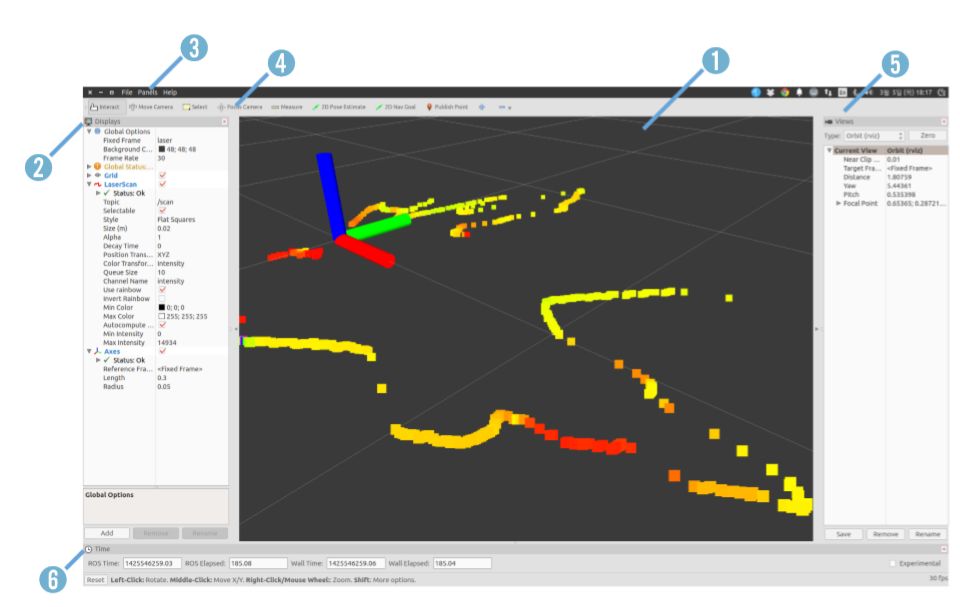
\includegraphics[width=1\linewidth]{src/C.png}
    \centering
    \caption{RViz画面布局} \label{picture:C}
\end{figure}

\begin{enumerate}
    \item 3D视图(3D view): 指屏幕的黑色部分。它是可以用三维方式查看各种数据的主屏幕。3D视图的背景颜色、固定框架、网格等可以在左侧显示的全局选项(Global Options)和网格(Grid)项目中进行详细设置。
    \item 显示屏(Displays): 左侧的显示屏是从各种话题当中选择用户所需的数据的视图的区域。如果单击屏幕左下方的[Add],选择屏幕将如RViz显示屏的选择画面所示。目前有大约30种不同的显示屏可供选择,我们将在下面的描述中详细介绍。
    \item 菜单(Menu): 菜单位于顶部。用户可以选择保存或读取显示屏状态的命令,还可以选择各种面板。
    \item 工具(Tools): 工具是位于菜单下方的按钮,允许用户用各种功能按键选择多种功能的工具,例如 Interact、Move Camera、Select,Focus Camera、Measure、2D Pose Estimate、2D Navigation Goal 以及Publish Point等。
    \item 视图(Views): 设定三维视图的视点。[Orbit:以指定的视点(在这里称为Focus)为中心旋转。这是默认情况下最常用的基本视图。]、[FPS(第一人称):显示第一人称视点所看到的画面。]、[ThirdPersonFollower:显示以第三人称的视点尾追特定目标的视图。]、[TopDownOrtho:这是Z轴的视图,与其他视图不同,以直射视图显示,而非透视法。]、[XYOrbit:类似于Orbit的默认值,但焦点固定在Z轴值为0的XY平面上。] 
    \item  时间(Time): 显示当前时刻(wall time)、ROS Time以及他们各自经过的时间。这主要用于仿真,如果需要重新启动,请点击底部的[Reset]按钮。
\end{enumerate}

\begin{figure}[htbp]
    \centering
    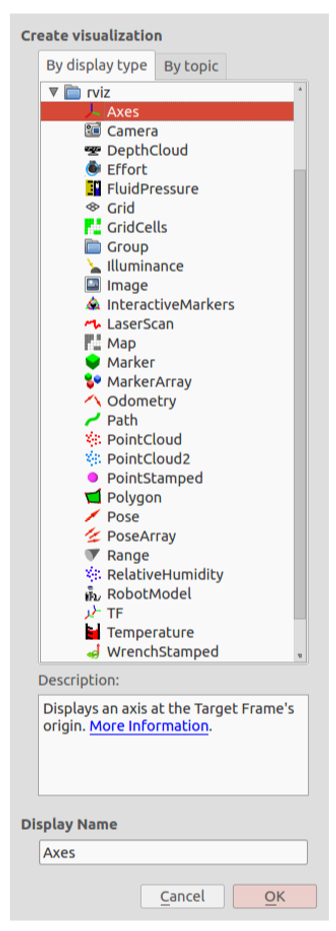
\includegraphics[width=0.45\linewidth]{src/D.png}
    \centering
    \caption{} \label{picture:}
\end{figure}
\subsubsection{RViz显示屏}
使用RViz的过程中最常用的菜单应该是显示屏菜单。该显示屏菜单用于选择三维视图(3D View)画面所显示的信息,各项目的说明请参照图E、F。

\begin{figure}[htbp]
    \centering
    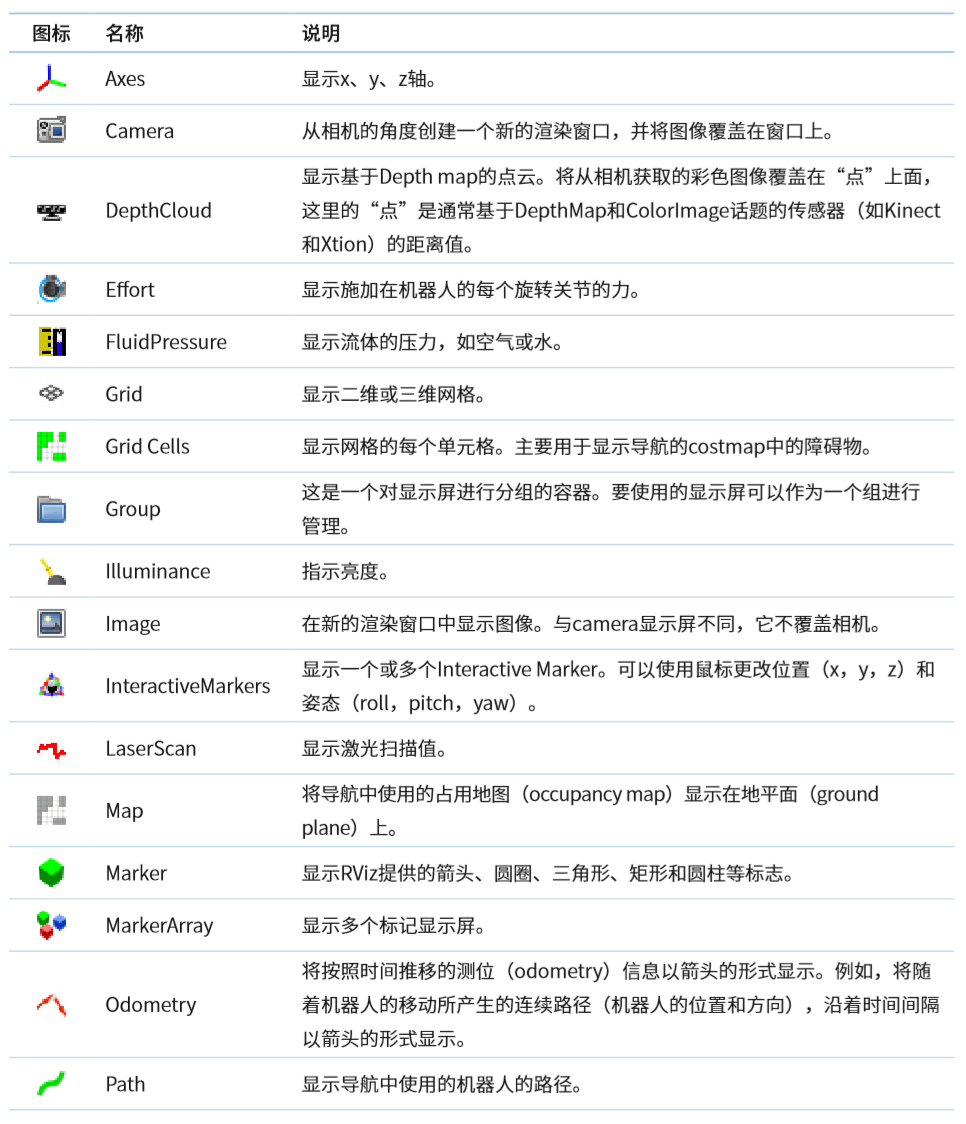
\includegraphics[width=1\linewidth]{src/E.png}
    \centering
    \caption{E} \label{picture:E}
\end{figure}

\begin{figure}[htbp]
    \centering
    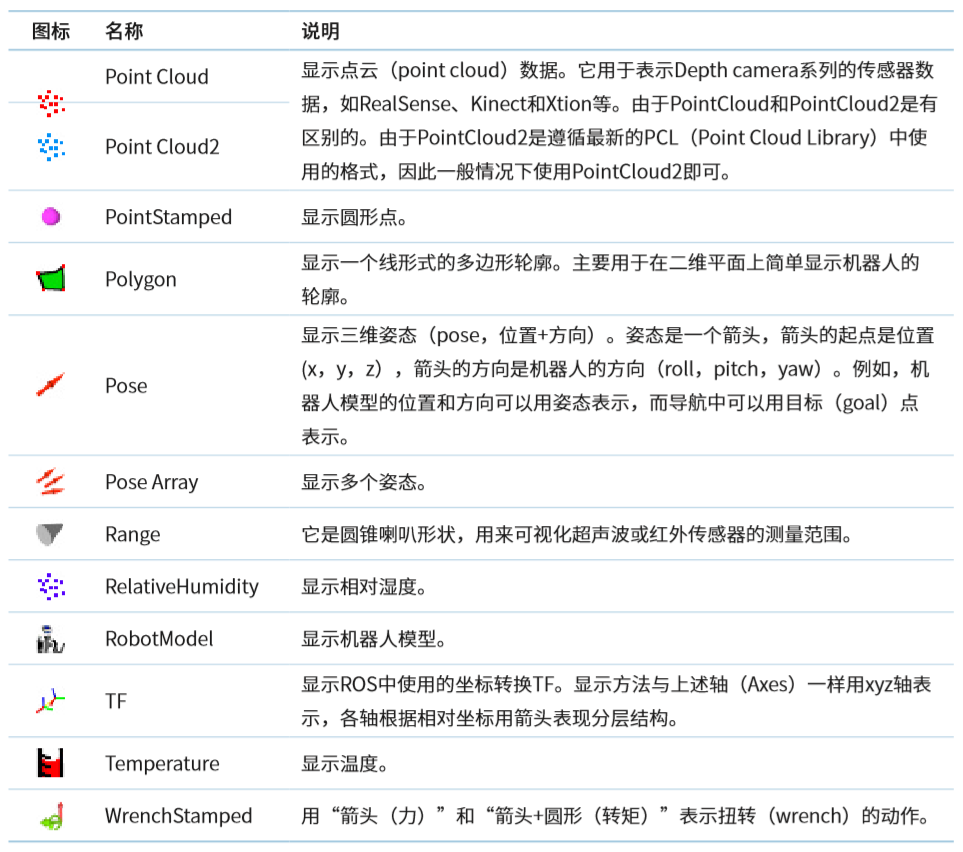
\includegraphics[width=1\linewidth]{src/F.png}
    \centering
    \caption{F} \label{picture:F}
\end{figure}
\subsection{ROSGUI开发工具(rqt)}
除了三维可视化工具RViz之外,ROS还为机器人开发提供各种GUI工具。例如,有一个将每个节点的层次结构显示为图形,且显示当前节点和话题状态的graph;将消息显示为二维图形的plot等。从ROS Fuerte版本开始,这些GUI开发工具被称为rqt6,它集成了30多种工具,可以作为一个综合的GUI工具来使用。另外,RViz也被集成到rqt的插件中,这使rqt成为ROS的一个不可缺少的GUI工具。

另外,顾名思义,rqt是基于Qt开发的,而Qt是一个广泛用于计算机编程的GUI编程的跨平台框架,用户可以方便自由地添加和开发插件。本节介绍rqt插件中的rqt\_image\_view、rqt\_graph、rqt\_plot和rqt\_bag。 
\subsubsection{rqt安装与运行}
运行rqt的命令如下。只需键入rqt。作为参考,用户可以使用节点执行命令“rosrun rqt\_gui rqt\_gui”执行它。 
\begin{lstlisting}[frame=single,language=]
    $ rqt
\end{lstlisting}

运行rqt将显示rqt的GUI界面,如下图所示。如果是第一次,它将只显示菜单,此外 没有任何内容。这是因为还没有指定rqt直接运行的插件程序。
\begin{figure}[htbp]
    \centering
    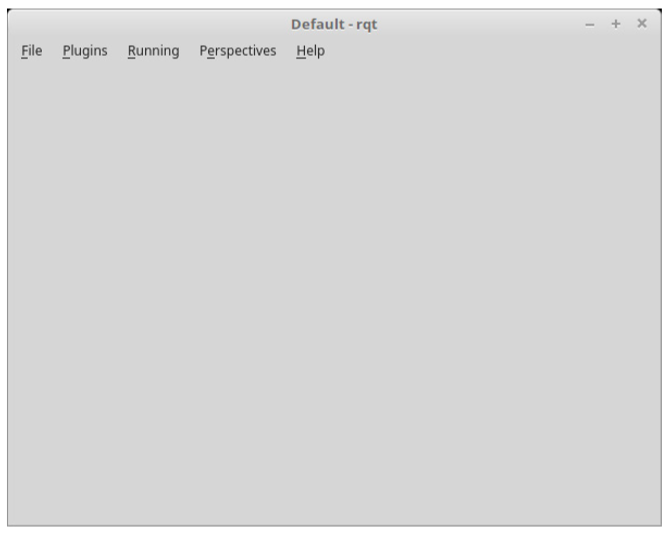
\includegraphics[width=1\linewidth]{src/G.png}
    \centering
    \caption{G} \label{picture:G}
\end{figure}

rqt的各菜单如下。

文件(File)  只有一个退出rqt的子菜单。

插件(Plugins) 有30多个插件。可以选择并使用它。

动作(Running) 显示当前运行的插件,在不需要的时候可以停止。

全景(Perspectives) 用于保存当前运行的插件组,并在下次运行相同的插件组。 
\subsubsection{rqt插件}
如果从rqt的顶部菜单中选择[插件(Plugins)],则可以看到大约30个插件。该插件具有以下功能。大部分是非常有用的rqt的默认插件。非官方的插件也可以添加到此,需要的话用户也可以添加自己开发的rqt插件。

动作(Action)

Action Type Browser: 查看动作类型的数据结构的插件。 

配置(Configuration)

Dynamic Reconfigure: 这是用于更改节点参数值的插件。

Launch: roslaunch的GUI插件,当不记得roslaunch的名称或配置时,它非常有用。

自检(Introspection)

Node Graph: 一种图形视图类型的插件,可以检查当前运行中的节点间的关系图与消息的流动。

Package Graph: 这是一个图形视图插件,显示功能包的依赖关系。

Process Monitor: 可以检查当前正在运行的节点的PID(进程ID)、CPU利用率、内存使用情况和线程数。

日志(Logging)

Bag: 是一个与ROS数据记录相关的插件。

Console: 它是一个允许用户在一个屏幕中查看来自节点的警告(Warning)和错误(Error)等消息的插件。

Logger Level: 通过选择负责发布日志的记录器节点来设置Debug、Info、Warn、Error和Fatal等日志信息(称为记录器级别)的工具。调试时选择Debug会非常方便。 

多种工具(Miscellaneous Tools)

Python Console: Python控制台屏幕插件。

Shell: 它是一个运行shell的插件。

Web: 运行Web浏览器的插件。 机器人工具(Robot Tools)

Controller Manager: 这是一个允许用户检查机器人控制器的状态、类型和硬件接口信息插件。

Diagnostic Viewer: 这是一个检查机器人设备和错误的插件。

Moveit! Monitor: 用于查看运动规划的MoveIt!数据的插件。

Robot Steering: 手动控制机器人的GUI工具。在远程控制时,利用此GUI工具进行机器人遥控会非常有用。

Runtime Monitor: 它是一个可以实时查看节点中发生的警告或错误的插件。

服务(Services)

Service Caller: 它是一个GUI插件,可以连接到正在运行中的服务服务器,并请求服务。这对测试服务(Service)很有用。

Service Type Browser: 这是一个用于检查服务类型的数据结构的插件。

话题(Topics)

Easy Message Publisher: 这是一个允许用户在GUI环境中发布话题的插件。

Topic Publisher: 这是一个可以发布话题的GUI插件,这对话题测试很有用。

Topic Type Browser: 这是检查话题类型的数据结构的插件。这对于检查话题类型很有用。

Topic Monitor: 这是一个列出当前正在使用的话题,并确认用户选择的话题信息的插件。

可视化(Visualization)

Image View: 这是一个可以检查相机的图像数据的插件。这对于简单的照相机数据测试非常有用。

Navigation Viewer: 这是一个用于在导航中检查机器人的位置和目标点的插件。

Plot: 这是一个绘图二维数据的GUI插件。这对于二维数据绘图非常有用。

Pose View: 它是一个显示机器人模型和TF的姿态(pose,位置和方向)的插件。

RViz: 这是RViz插件,是一个3D可视化工具插件。

TF Tree: 这是一个图形视图插件,它用树形图显示了通过TF收集的每个坐标之间的关系。

\begin{figure}[htbp]
    \centering
    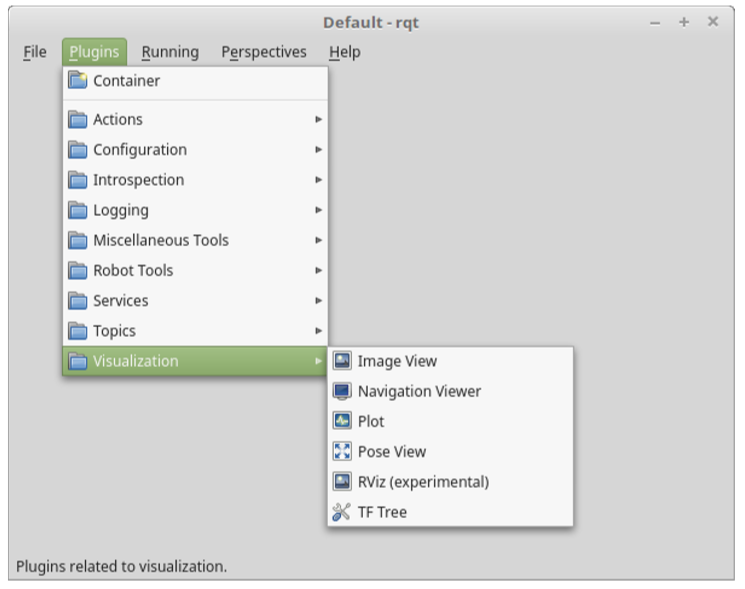
\includegraphics[width=1\linewidth]{src/H.png}
    \centering
    \caption{H} \label{picture:H}
\end{figure}
\subsubsection{Rqt\_image\_view}
这是一个显示相机的图像数据的插件。这不是一个图像处理过程,它只是在简单地查看图像时非常有用。一般的USB摄像头支持UVC,所以用户可以使用ROS的uvc\_camera功能包。首先,使用以下命令安装uvc\_camera功能包。
\begin{lstlisting}[frame=single,language=]
    $ sudo apt-get install ros-kinetic-uvc-camera
\end{lstlisting}

将USB摄像头连接到计算机的USB接口,然后使用以下命令运行uvc\_camera功能包中的uvc\_camera\_node节点。
\begin{lstlisting}[frame=single,language=]
    $ rosrun uvc_camera uvc_camera_node
\end{lstlisting}

然后用“rqt”命令运行rqt,之后从菜单中选择[Plugins]→[Image View]。如果在左上方的消息选择下拉列表中选择“/image\_raw”,则可以看到如图6-10所示的图像。
\begin{lstlisting}[frame=single,language=]
    $ rqt 
\end{lstlisting}

\begin{figure}[htbp]
    \centering
    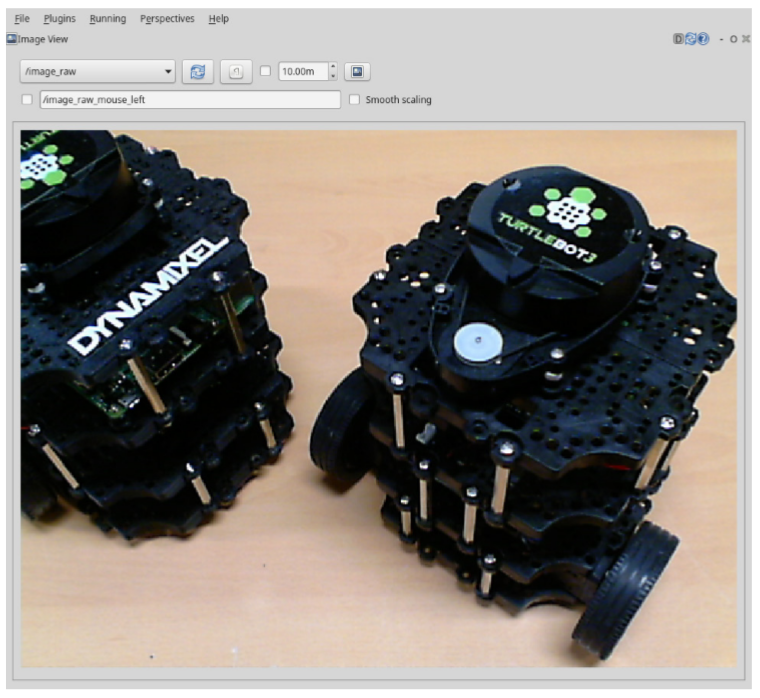
\includegraphics[width=1\linewidth]{src/I.png}
    \centering
    \caption{I} \label{picture:I}
\end{figure}

除了从rqt菜单中选择插件之外,还可以使用专用的运行命令,如下所示。
\begin{lstlisting}[frame=single,language=]
    $ rqt_image_view
\end{lstlisting}
\subsubsection{rqt\_graph}
rqt\_graph是用图形表示当前活动中的节点与在ROS网络上传输的消息之间的相关性的工具。这对了解当前ROS网络情况非常有用。用法很简单。如以下示例所示,为了查看第3.3节中描述的turtlesim功能包中的turtlesim\_node和turtle\_teleop\_key,以及第6.2.3节中描述的uvc\_camera功能包中的uvc\_camera\_node节点,将他们分别在不同的终端中运行。 
\begin{lstlisting}[frame=single,language=]
    $ rosrun turtlesim turtlesim_node 
    $ rosrun turtlesim turtle_teleop_key 
    $ rosrun uvc_camera uvc_camera_node 
    $ rosrun image_ view image_view image:=image_raw
\end{lstlisting}

然后如下例所示,使用命令“rqt”运行rqt并从菜单中选择[Plugins]→[Node Graph]即可。请注意,用户也可以在终端中运行“rqt\_graph”,而无需直接从菜单中选择插件。运行rqt\_graph时,节点和话题的相关性会如图6-11所示显示。
\begin{lstlisting}[frame=single,language=]
    $ rqt
\end{lstlisting} 

\begin{figure}[htbp]
    \centering
    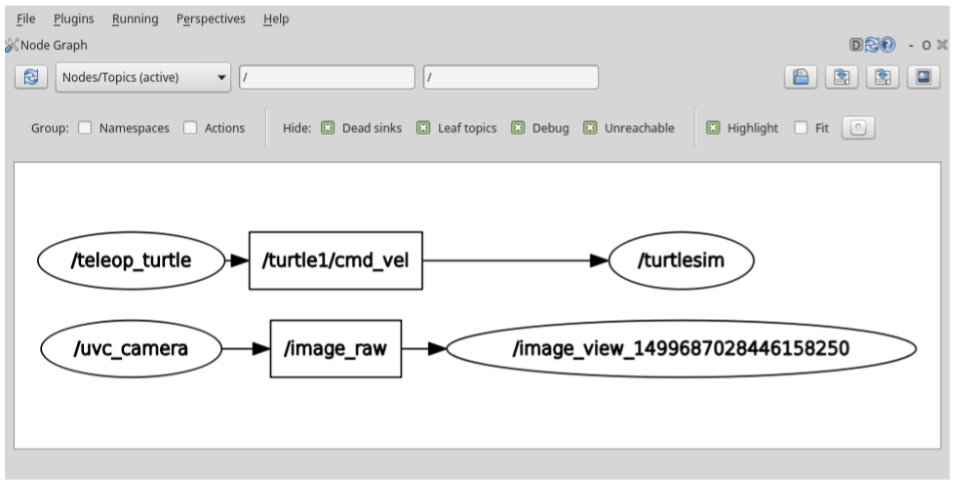
\includegraphics[width=1\linewidth]{src/J.png}
    \centering
    \caption{J} \label{picture:J}
\end{figure}

在图6-11中,椭圆表示节点(/teleop\_turtle、/turtlesim),方块(/turtle1/cmd\_vel)表示话题消息。箭头表示发送和接收消息。在前面的例子中,运行turtle\_teleop\_key时,会运行teleop\_turtle节点;运行turtlesim\_node节点时,会运行turtlesim节点。可以看到,这两个节点正在以平移速度和旋转速度的消息类型(话题名称:/turtle1/ cmd\_vel)发送和接收键盘的方向键值。uvc\_camera功能包也可以通过rqt\_graph确认uvc\_camera节点在发出/image\_raw 话题消息,并且image\_view\_xxx节点在订阅它。这已经通过简单的几个节点确认过,但在实际的ROS编程中,会有数十个节点发送和接收各种话题消息。此时,rqt\_graph对于检查当前ROS网络上节点的相关性会非常的有用。
\subsubsection{rat\_plot}
这一次,我们使用下面的命令运行rqt\_plot,而不是在rqt界面中选择插件。作为参考,用户可以使用节点执行命令rosrun rqt\_plot rqt\_plot运行它。 

\begin{lstlisting}[frame=single,language=]
    $ rqt_plot 
\end{lstlisting}

rqt\_plot运行后,点击程序右上角的齿轮形状的选项图标。可以如图6-12所示选择一个选项,其默认设置为“MatPlot”。除MatPlot外,还提供了PyQtGraph和QwtPlot。请参阅相关的安装说明并使用所需的图形库。例如,如果要使用PyQtGraph作为默认绘图而不是MatPlot,请从以下下载地址下载并安装最新的python-pyqtgraph\_0.9.xx-x\_all.deb文件。安装PyQtGraph之后,用户可以使用PyQtGraph。

\begin{figure}[htbp]
    \centering
    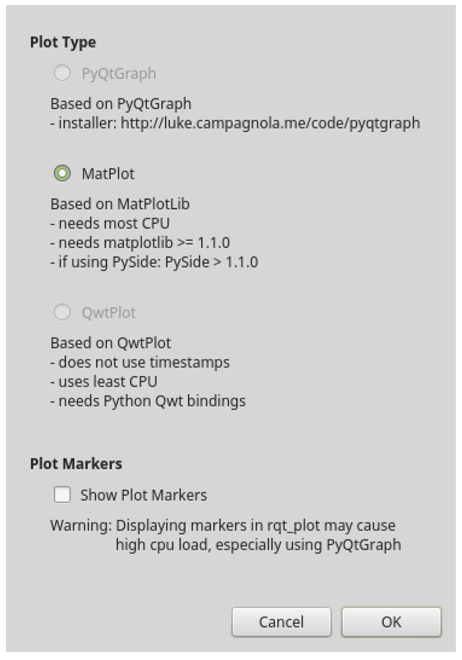
\includegraphics[width=0.8\linewidth]{src/K.png}
    \centering
    \caption{K} \label{picture:K}
\end{figure}

rqt\_plot是一个二维数据绘图工具。绘图意味着绘制坐标。换句话说,它接收到ROS消息并将其撒在坐标系上。例如,假设要标记turtlesim节点pose消息的x和y坐标。首先,运行turtlesim功能包中的turtlesim\_node。
\begin{lstlisting}[frame=single,language=]
    $ rosrun turtlesim turtlesim_node
\end{lstlisting}

然后在rqt\_plot上方的Topic栏中输入/turtle1/pose/,则会在二维(x轴:数据值, y轴:时间)坐标系中绘制/turtle1/pose/节点。或者,您可以使用下一个命令立即运行它,包括指定要图示的话题。
\begin{lstlisting}[frame=single,language=]
    $ rqt_plot /turtle1/pose/
\end{lstlisting}

接下来,运行turtlesim功能包中的turtle\_teleop\_key来移动屏幕上的乌龟。
\begin{lstlisting}[frame=single,language=]
    $ rosrun turtlesim turtle_teleop_key
\end{lstlisting}

如图6-13所示,可以看到在显示龟的x位置、y位置、theta方向和平移转速。这是显示二维数据坐标的有用的工具。这里表示了turtlesim功能包,但rqt\_plot也可以用于表达用户开发的节点的二维数据。特别地,适合于随着时间的推移显示传感器值,例如速度和加速度。

\begin{figure}[htbp]
    \centering
    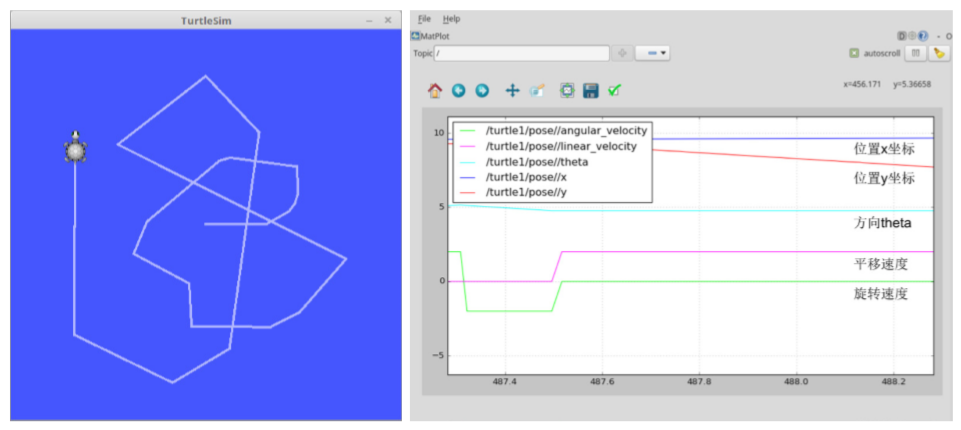
\includegraphics[width=1\linewidth]{src/L.png}
    \centering
    \caption{L} \label{picture:L}
\end{figure}
\subsubsection{rqt\_bag}
rqt\_bag是一个可以将消息进行可视化的GUI工具。在5.4.8节中,ROS日志信息中的rosbag是基于文本的,但是rqt\_bag对于图像数据类的消息管理是非常有用的,因为rqt\_bag多了可视化功能,因此可以立即查看摄像机的图像值。在测试之前,运行rqt\_image\_view和rqt\_graph的工具说明中提到的turtlesim和uvc\_camera中的所有相关节点。接下来,用如下命令生成为一个bag文件,记录相机的/image\_raw和turtlesim的/turntlesim/turtle1/cmd\_vel值。

在第5.4节中,曾使用rosbag程序将ROS上的各种话题消息作为bag文件进行保存、回放和压缩。rqt\_bag是rosbag的GUI版本,和rosbag一样,它可以存储、回放和压缩话题消息。另外,由于它是一个GUI程序,所有的命令都是用按钮制作的,所以它很容易使用,并且用户可以用类似使用视频编辑器一样,在时间轴上来回查看摄像机图像。

为了利用rqt\_bag的特点,将USB摄像头图像保存为一个bag文件,然后使用rqt\_bag 进行播放。
\begin{lstlisting}[frame=single,language=]
    $ rosrun uvc_camera uvc_camera_node 
    $ rosbag record /image_raw 
    $ rqt 
\end{lstlisting}

使用“rqt”命令运行rqt,然后从菜单中选择[插件(Plugins)]→[日志 (Logging)]→[包(Bag)]。然后选择左上方的文件夹图标(Load Bag)加载刚才 录制的*.bag文件。然后,如图6-14所示,用户可以在时间轴上查看相机图像的变化。 还可以进行放大、回放和查看各时间点的数据值。如果右键单击鼠标按钮,则会出现“Publish”选项来重新发送消息。

\begin{figure}[htbp]
    \centering
    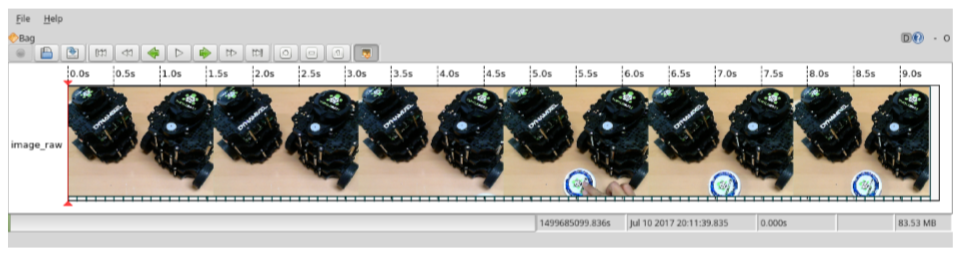
\includegraphics[width=1\linewidth]{src/M.png}
    \centering
    \caption{M} \label{picture:M}
\end{figure}
\section{ROS编程基础}
\subsection{ROS编程前须知事项}
\subsubsection{标准单位}
对ROS中所使用的消息(message),推荐使用世界上最广泛运用的标准单位SI。为了确保这一点,REP-0103也明确了各物理量的单位。

例如,长度(Length)使用米(merter)、质量(Mass)使用千克(Kilogram)、时间(Time)使用秒(Second)、电流(Current)使用安培(Ampere)、角度(Angle)使用弧度(Radian)、频率(Frequency)使用赫兹(Hertz)、力(Force)使用牛顿(Newton)、功率(Power)使用瓦(Watt)、电压(Voltage)使用伏特(Volt)、温度(Temperature)使用摄氏度(Celsius)。其他所有单位都是这些单位的组合。

消息鼓励重用ROS提供的方式,但也可以根据需要使用用户全新定义的新的类型的消息。然而,消息用到的单位却必须要遵守使用SI单位,这是为了让其他用户使用这种消息的时候不需要转换单位。

REP(ROS Enhancement Proposals):REP是一份建议书,它的内容包含由用户们在ROS社区提出的规则、新功能和管理方法。它用于以民 主方式创建ROS的规则的情况,还用于在协商ROS的开发、运营和管理所需的内容的情况。收到建议 书后,许多ROS用户可以查看,并通过互相协商继续修改。REP就是通过这样的过程成为ROS标准文 档的。REP文件的目录可以在http://www.ros.org/reps/rep-0000.html 找到。
\subsubsection{坐标表现方式}
如图左侧所示,ROS中的旋转轴使用x,y和z轴。正面是x轴的正方向,轴是红色(R)。左边是y轴的正方向,轴用绿色(G)表示。最后,上方是z轴的正方向,轴用蓝色(B)表示。为了便于记忆,您可以将x轴视为食指,将y轴视为中指,将z轴视为拇 指。顺序是x、y、z,且颜色是RGB颜色顺序。机器人的旋转方向是右手定则,用右手卷住的方向是正(+)方向。这种坐标表示法在ROS编程中经常使用,必须以x:forward,y:left,z:up的形式进行编程。
\begin{figure}[htbp]
    \centering
    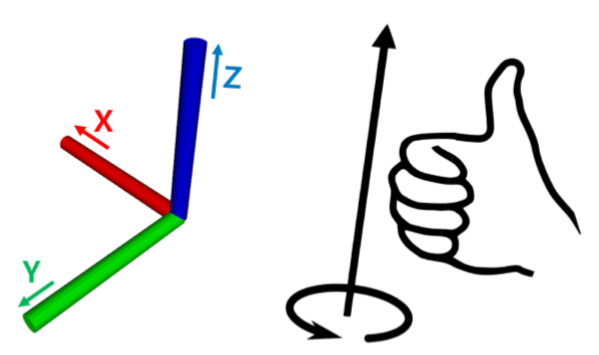
\includegraphics[width=1\linewidth]{src/N.png}
    \centering
    \caption{N} \label{picture:N}
\end{figure}

\subsubsection{编程规则}
为了最大化每个程序的源代码的可重用性,ROS指定了编程风格指南,并建议开发者遵守该指南。这减少了开发人员在处理源代码时频繁发生的额外的选项,也提高了其他协作开发人员和用户们的代码理解程度,并降低了他们之间的代码分析难度。这不是一个要求,但为了代码共享,笔者想鼓励ROS的许多用户遵守这一规则。编程规则在wiki(C++,Python)中按各个编程语言有详细解释。下面的表格中整理了基本的命名规则。
\begin{figure}[htbp]
\centering
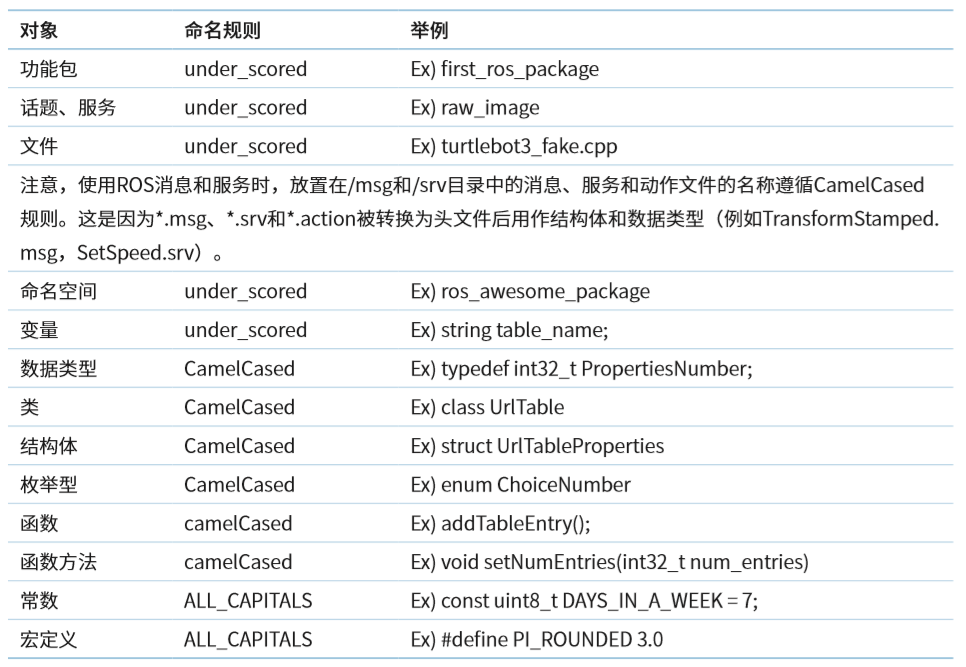
\includegraphics[width=1\linewidth]{src/O.png}
\centering
\caption{O} \label{picture:O}
\end{figure}

\subsection{发布者节点和订阅者节点的创建和运行}
ROS消息通信中使用的发布者(Publisher)和订阅者(Subscriber)可以被发送和接收所代替。在ROS中,发送端称为发布者,接收端称为订阅者。本节旨在创建一个简单的msg文件,并创建和运行发布者和订阅者节点。 
\subsubsection{创建功能包}
以下命令是创建ros\_tutorials\_topic功能包的命令。这个功能包依赖于message\_generation、std\_msgs和roscpp功能包,因此将这些用作依赖选项。第二行命令意味着将使用创建新的功能包时用到的message\_generation表示将使用创建新消息的功能包std\_msgs(ROS标准消息功能包)和roscpp(在ROS中使用C/C ++的客户端程序库)必须在创建功能包之前安装。用户可以在创建功能包时指定这些相关的功能包设置,但也可以在创建功能包之后直接在package.xml中修改。
\begin{lstlisting}[frame=single,language=]
    $ cd ~/catkin_ws/src 
    $ catkin_create_pkg ros_tutorials_topic message_generation std_msgs roscpp 
\end{lstlisting}

创建功能包时,将在~/catkin\_ws/src目录中创建ros\_tutorials\_topic功能包目录,并在该功能包目录中创建ROS功能包的默认目录和CMakeLists.txt和package.xml文件。可以使用下面的ls命令检查它,并使用基于GUI的Nautilus(类似Windows资源管理器)来检查功能包的内部。 
\begin{lstlisting}[frame=single,language=]
    $ cd ros_tutorials_topic 
    $ ls 
    include   → 头文件目录 
    src     → 源代码目录 
    CMakeLists.txt   → 构建配置文件 
    package.xml    → 功能包配置文件 
\end{lstlisting}
\subsubsection{修改功能包配置文件}
ROS的必备配置文件package.xml是一个包含功能包信息的XML文件,其中包含用于描述功能包名称、作者、许可证和依赖包的信息。使用以下命令,利用编辑器(gedit、vim、emacs等)打开文件,并修改它以匹配当前节点。以下是本次Demo:
\begin{lstlisting}[frame=single,language=xml]
    <?xml version="1.0"?> 
    <package>  
    <name>ros_tutorials_topic</name>  
    <version>0.1.0</version>  
    <description>ROS tutorial package to learn the topic</description>  
    <license>Apache License 2.0</license>  
    <author email="pyo@robotis.com">Yoonseok Pyo</author>  
    <maintainer email="pyo@robotis.com">Yoonseok Pyo</maintainer>  
    <url type="bugtracker">https://github.com/ROBOTIS-GIT/ros_tutorials/issues</url>  
    <url type="repository">https://github.com/ROBOTIS-GIT/ros_tutorials.git</url>  
    <url type="website">http://www.robotis.com</url>  
    <buildtool_depend>catkin</buildtool_depend>  
    <build_depend>roscpp</build_depend>  
    <build_depend>std_msgs</build_depend>  
    <build_depend>message_generation</build_depend>  
    <run_depend>roscpp</run_depend>  
    <run_depend>std_msgs</run_depend>  
    <run_depend>message_runtime</run_depend>  
    <export></export> 
    </package>
\end{lstlisting}
\subsubsection{修改构建配置文件(Cmakelists.txt)}
ROS的构建系统catkin基本上使用CMake,它在功能包目录中的CMakeLists.txt文件中描述了构建环境。该文件设置可执行文件的创建、依赖包优先构建、链接创建等。以下是本此的Demo:
\begin{lstlisting}[frame=single,language=]
    cmake_minimum_required(VERSION 2.8.3) 
    project(ros_tutorials_topic) 
    
    ## catkin构建时需要的组件包。 
    ## 是依赖包,是message_generation、 std_msgs和roscpp。 
    ## 如果这些功能包不存在,在构建过程中会发生错误。 
    find_package(catkin REQUIRED COMPONENTS message_generation std_msgs roscpp) 
    
    ## 消息声明:MsgTutorial.msg 
    add_message_files(FILES MsgTutorial.msg) 
    
    ## 这是设置依赖性消息的选项。 
    ## 如果未安装std_msgs,则在构建过程中会发生错误。 
    generate_messages(DEPENDENCIES std_msgs) 
    
    ## catkin功能包选项,描述了库、catkin构建依赖项和系统依赖的功能包。 
    catkin_package(      
        LIBRARIES ros_tutorials_topic    
        CATKIN_DEPENDS std_msgs roscpp 
    )
    
    ## 设置包含目录。 
    include_directories(${catkin_INCLUDE_DIRS}) 
    
    ## topic_publisher节点的构建选项。 
    ## 配置可执行文件、目标链接库和其他依赖项。 
    add_executable(topic_publisher src/topic_publisher.cpp) 
    add_dependencies(topic_publisher ${${PROJECT_NAME}_EXPORTED_TARGETS} ${catkin_EXPORTED_TARGETS}) 
    target_link_libraries(topic_publisher ${catkin_LIBRARIES}) 
    
    ## topic_subscriber节点的构建选项。 
    add_executable(topic_subscriber src/topic_subscriber.cpp) 
    add_dependencies(topic_subscriber ${${PROJECT_NAME}_EXPORTED_TARGETS} ${catkin_EXPORTED_TARGETS}) 
    target_link_libraries(topic_subscriber ${catkin_LIBRARIES})
\end{lstlisting}
\subsubsection{创建消息文件}
在上述的CMakeLists.txt文中添加了如下选项。 
\begin{lstlisting}[frame=single,language=]
    add_message_files(FILES MsgTutorial.msg)
\end{lstlisting}

这意味着在构建时要包含消息MsgTutorial.msg,该消息将在此节点中被使用。现在我们还没有创建MsgTutorial.msg,因此按以下顺序创建它: 
\begin{lstlisting}[frame=single,language=]
    $ roscd ros_tutorials_topic  → 移动到功能包目录 
    $ mkdir msg       → 功能包中创建新的msg消息目录 
    $ cd msg       → 转到创建的msg目录 
    $ gedit MsgTutorial.msg    → 创建新的MsgTutorial.msg文件并修改内容
\end{lstlisting}

内容很简单。如下所示,创建一个time消息类型的stamp消息和一个int32消息类型的data消息,除了这些消息类型之外,还有一些如bool、int8、int16、float32、string、time、duration和common\_msgs等基本消息类型,以及在ROS中收集常用消息的common\_msgs。这里我们只是为了创建一个简单的例子,因此用了time和int32。以下是文件内容:
\begin{lstlisting}[frame=single,language=]
    time stamp 
    int32 data
\end{lstlisting}

消息(msg、srv、action)功能包的独立化:一般情况下,建议将消息文件msg和服务文件srv制作成一个只包含消息文件的单独的包,而不是将其包含在可执行节点中。其原因是,假设订阅者节点和发布者节点在不同的计算机上运行,存在的问题是必须安装不必要的节点,因为这两个节点只有在它们具有相互依赖性时才能使用。如果您独立创建消息功能包,则只需将独立于消息的功能包添加到依赖性选项,从而消除功能包之间不必要的依赖关系。但是,在本书中,我们为了简化代码已经将消息文件包含在可执行节点中。
\subsubsection{创建发布者节点}
在前面的CMakeLists.txt文件中,给了生成以下可执行文件的选项。
\begin{lstlisting}[frame=single,language=]
    add_executable(topic_publisher src/topic_publisher.cpp)
\end{lstlisting}

换句话说,是在src目录中构建topic\_publisher.cpp文件以创建topic\_publisher可执行文件。那么我们按如下顺序创建一个执行发布者节点函数的源代码。
\begin{lstlisting}[frame=single,language=]
    $ roscd ros_tutorials_topic/src   → 移至src目录,该目录是功能包的源代码目录 
    $ gedit topic_publisher.cpp    → 新建源文件并修改内容
\end{lstlisting}

以下是此cpp文件内容:
\begin{lstlisting}[frame=single,language=C++]
    #include "ros/ros.h"     // ROS默认头文件 
    #include "ros_tutorials_topic/MsgTutorial.h"  // MsgTutorial消息头文件(构建后自动生成) 
    int main(int argc, char **argv)    // 节点主函数 
    {  
        ros::init(argc, argv, "topic_publisher");  // 初始化节点名称  
        ros::NodeHandle nh;     // 声明一个节点句柄来与ROS系统进行通信  
        
        // 声明发布者,创建一个使用ros_tutorials_topic功能包的MsgTutorial消息文件的  
        // 发布者ros_tutorial_pub。话题名称是"ros_tutorial_msg",  
        // 消息文件发布者队列(queue)的大小设置为100      
        ros::Publisher ros_tutorial_pub = nh.advertise<ros_tutorials_topic::MsgTutorial>("ros_tutorial_msg", 100); 
        
        // 设定循环周期。"10"是指10Hz,是以0.1秒间隔重复  
        ros::Rate loop_rate(10);  
        
        ros_tutorials_topic::MsgTutorial msg; // 以MsgTutorial消息文件格式声明一个叫做msg的消息  
        
        int count = 0;                             // 声明要在消息中使用的变量  
        
        while (ros::ok())  {    
            msg.stamp = ros::Time::now();   // 把当前时间传给msg的下级消息stamp     
            msg.data  = count;     // 将变量count的值传给下级消息data
            ROS_INFO("send msg = %d", msg.stamp.sec);   // 显示stamp.sec消息    
            ROS_INFO("send msg = %d", msg.stamp.nsec);  // 显示stamp.nsec消息    
            ROS_INFO("send msg = %d", msg.data);        // 显示data消息    
            ros_tutorial_pub.publish(msg);  // 发布消息。    
            loop_rate.sleep();    // 按照上面定义的循环周期进行暂歇    
            ++count;      // 变量count增加1  
        }  
        return 0; 
    }
\end{lstlisting}
\subsubsection{创建订说者节点}
在CMakeLists.txt文件中添加以下选项来生成可执行文件。
\begin{lstlisting}[frame=single,language=]
    add_executable(topic_subscriber src/topic_subscriber.cpp) 
\end{lstlisting}

也就是说,通过构建topic\_subscriber.cpp文件来创建topic\_subscriber可执行文件。我们创建一个按照以下顺序执行订阅节点功能的源代码。
\begin{lstlisting}[frame=single,language=]
    $ roscd ros_tutorials_topic/src  → 移动到src目录,该目录是功能包的源代码目录 
    $ gedit topic_subscriber.cpp   → 创建和修改新的源代码文件
\end{lstlisting}

以下是此cpp文件内容:
\begin{lstlisting}[frame=single,language=]
    #include "ros/ros.h"     // ROS的默认头文件 
    #include "ros_tutorials_topic/MsgTutorial.h"  // MsgTutorial消息头文件(构建后自动生成) 
    
    // 这是一个消息后台函数, 
    // 此函数在收到一个下面设置的名为ros_tutorial_msg的话题时候被调用。 
    // 输入的消息是从ros_tutorials_topic功能包接收MsgTutorial消息。 
    
    void msgCallback(const ros_tutorials_topic::MsgTutorial::ConstPtr& msg)
    { 
        ROS_INFO("recieve msg = %d", msg->stamp.sec);  // 显示stamp.sec消息  
        ROS_INFO("recieve msg = %d", msg->stamp.nsec);  // 显示stamp.nsec消息  
        ROS_INFO("recieve msg = %d", msg->data);  // 显示data消息 
    } 
    
    int main(int argc, char **argv)   // 节点主函数 
    {  
        ros::init(argc, argv, "topic_subscriber");  // 初始化节点名称   
        ros::NodeHandle nh;                        // 声明用于ROS系统和通信的节点句柄  
        
        // 声明订阅者,创建一个订阅者ros_tutorial_sub,  
        // 它利用ros_tutorials_topic功能包的的MsgTutorial消息文件。  
        // 话题名称是"ros_tutorial_msg",订阅者队列(queue)的大小设为100。  
        ros::Subscriber ros_tutorial_sub = nh.subscribe("ros_tutorial_msg", 100, msgCallback);  
        
        // 用于调用后台函数,等待接收消息。在接收到消息时执行后台函数。  
        ros::spin();  
        
        return 0; 
    }
\end{lstlisting}

之后执行:
\begin{lstlisting}[frame=single,language=]
    $ cd ~/catkin_ws    → 移动到catkin目录 
    $ catkin_make    → 执行catkin构建 
\end{lstlisting}
\subsubsection{构建(build)节点}
现在使用以下命令在ros\_tutorials\_topic功能包中构建消息文件、发布者节点和订阅者节点。ros\_tutorials\_topic功能包的源代码位于“~/catkin\_ws/src/ros\_tutorials\_topic/src”中,而ros\_tutorials\_topic功能包中的消息文件位于“~/catkin\_ws/src/ros\_tutorials\_topic/msg”中。 基于此的构建将分别在“~/catkin\_ws”的“/build”和“/devel”目录中生成文件。“/build”目录中保存catkin构建用到的配置内容,而“/devel/lib/ros\_tutorials\_topic’”目录中保存可执行文件。另外,“/devel/include/ros\_tutorials\_topic”目录存储着从消息文件自动生成的消息头文件。如果您想了解生成文件,请根据目录查看文件。
\subsubsection{运行发布者}
以下是使用rosrun命令运行ros\_tutorials\_topic功能包的ros\_tutorial\_msg\_publisher节点的命令。运行节点之前,请确保要从另一个终端运行 roscore。在以下示例中,即使没有解释,roscore也必须在运行节点之前运行。
\begin{lstlisting}[frame=single,language=]
    $ roscore 
    $ rosrun ros_tutorials_topic topic_publisher
\end{lstlisting}

下面,我们使用rostopic命令获取topic\_publisher发布的话题吧。首先,我们来看 一下ROS网络当前正在使用的话题列表。通过将list选项添加到rostopic命令来查看是否 存在ros\_tutorial\_msg话题。
\begin{lstlisting}[frame=single,language=]
    $ rostopic list 
    /ros_tutorial_msg 
    /rosout 
    /rosout_agg 
\end{lstlisting}

接下来,让我们看看我们运行的发布者节点发布的消息。换句话说,是检查ros\_tutorial\_msg话题消息。您可以看到发布的消息。 
\begin{lstlisting}[frame=single,language=]
    $ rostopic echo /ros_tutorial_msg
\end{lstlisting}
\subsubsection{运行订阅者}
以下是为了运行订阅者使用ROS节点命令rosrun来运行ros\_tutorials\_topic功能包的topic\_subscriber节点的过程。 
\begin{lstlisting}[frame=single,language=]
    $ rosrun ros_tutorials_topic topic_subscriber
\end{lstlisting}

订阅者接收到了发布者发布的ros\_tutorial\_msg话题的消息,并在屏幕上显示该值。
\subsubsection{检查运行中的节点的通信状态}
让我们用6.2节中介绍的rqt命令来查看运行中的节点的通信状态。您可以使用rqt\_graph或rqt,如下所示。执行rqt时,在菜单中选择[Plugins]→[Introspection]→[Node Graph]可以确认当前在ROS上运行的节点和消息。
\begin{lstlisting}[frame=single,language=]
    $ rqt_graph 或 $ rqt 
\end{lstlisting}

在当前的ROS网络上,发布者节点(topic\_publisher)正在传输话题(ros\_tutorial\_msg),并且可以确认它正在接收订阅者节点(topic\_subscriber)。
\subsection{创建和运行服务服务器与客户端节点}
服务由服务服务器(service server)和服务客户端(service client)组成,其中服务服务器仅在收到请求(request)时才会响应(response),而服务客户端则会发送请求并接收响应。与话题不同,服务是一次性消息通信。因此,当服务的请求和响应完成 时,两个节点的连接会被断开。 这种服务通常在让机器人执行特定任务时用到。或者用于需要在特定条件下做出反应 的节点。由于它是一次性的通信方式,因此对网络的负载很小,所以是一种非常有用的通 信手段,例如被用作一种代替话题的通信手段。 本节旨在创建一个简单的服务文件,并创建和运行一个服务服务器(server)节点和一个服务客户端(client)节点。
\subsubsection{创建功能包}
以下命令是创建ros\_tutorials\_topic功能包的命令。这个功能包依赖于message\_generation、std\_msgs和roscpp功能包,因此将这些用作依赖选项。第二行命令意味着将使用创建新的功能包时用到的message\_generation表示将使用创建新消息的功能包std\_msgs(ROS标准消息功能包)和roscpp(在ROS中使用C/C ++的客户端程序库)必须在创建功能包之前安装。用户可以在创建功能包时指定这些相关的功能包设置,但也可以在创建功能包之后直接在package.xml中修改。
\begin{lstlisting}[frame=single,language=]
    $ cd ~/catkin_ws/src 
    $ catkin_create_pkg ros_tutorials_topic message_generation std_msgs roscpp 
\end{lstlisting}

创建功能包时,将在~/catkin\_ws/src目录中创建ros\_tutorials\_topic功能包目录,并在该功能包目录中创建ROS功能包的默认目录和CMakeLists.txt和package.xml文件。可以使用下面的ls命令检查它,并使用基于GUI的Nautilus(类似Windows资源管理器)来检查功能包的内部。 
\begin{lstlisting}[frame=single,language=]
    $ cd ros_tutorials_topic 
    $ ls 
    include   → 头文件目录 
    src     → 源代码目录 
    CMakeLists.txt   → 构建配置文件 
    package.xml    → 功能包配置文件 
\end{lstlisting}
\subsubsection{修改功能包配置文件(package.xml)}
内容如下:
\begin{lstlisting}[frame=single,language=xml]
    <?xml version="1.0"?> 
    <package>  
    <name>ros_tutorials_service</name>  
    <version>0.1.0</version>  
    <description>ROS tutorial package to learn the service</description>  
    <license>Apache License 2.0</license>  
    <author email="pyo@robotis.com">Yoonseok Pyo</author>  
    <maintainer email="pyo@robotis.com">Yoonseok Pyo</maintainer>  
    <url type="bugtracker">https://github.com/ROBOTIS-GIT/ros_tutorials/issues</url>  
    <url type="repository">https://github.com/ROBOTIS-GIT/ros_tutorials.git</url>  
    <url type="website">http://www.robotis.com</url>  
    <buildtool_depend>catkin</buildtool_depend>  
    <build_depend>roscpp</build_depend>  
    <build_depend>std_msgs</build_depend>  
    <build_depend>message_generation</build_depend>  
    <run_depend>roscpp</run_depend>  
    <run_depend>std_msgs</run_depend>  
    <run_depend>message_runtime</run_depend>  
    <export></export> 
    </package>
\end{lstlisting}
\subsubsection{修改构建配置文件(CMakelists.txt)}
内容如下:
\begin{lstlisting}[frame=single,language=]
    cmake_minimum_required(VERSION 2.8.3) 
    project(ros_tutorials_service) 
    
    ## 这是进行catkin构建时所需的组件包。 
    ## 依赖包是message_generation、std_msgs和roscpp。如果这些包不存在,在构建过程中会发生错误。 find_package(catkin REQUIRED COMPONENTS message_generation std_msgs roscpp) 
    
    ## 服务声明:SrvTutorial.srv 
    add_service_files(FILES SrvTutorial.srv) 
    
    ## 这是一个设置依赖消息的选项。 
    ## 如果未安装std_msgs,则在构建过程中会发生错误。 
    generate_messages(DEPENDENCIES std_msgs) 
    
    ## 这是catkin功能包选项,它描述了库、catkin构建依赖和依赖系统的功能包。 
    catkin_package(      
        LIBRARIES ros_tutorials_service    
        CATKIN_DEPENDS std_msgs roscpp 
    )
    
    ## 设置包含目录。 
    include_directories(${catkin_INCLUDE_DIRS}) 
    
    ## 这是service_server节点的构建选项。 
    ## 设置可执行文件、目标链接库和附加依赖项。 
    add_executable(service_server src/service_server.cpp) 
    add_dependencies(service_server ${${PROJECT_NAME}_EXPORTED_TARGETS} ${catkin_EXPORTED_TARGETS}) 
    target_link_libraries(service_server ${catkin_LIBRARIES}) 
    
    ## 这是节点的构建选项。 
    add_executable(service_client src/service_client.cpp) 
    add_dependencies(service_client ${${PROJECT_NAME}_EXPORTED_TARGETS} ${catkin_EXPORTED_TARGETS}) 
    target_link_libraries(service_client ${catkin_LIBRARIES})
\end{lstlisting}
\subsubsection{创建服务文件}
CMakeLists.txt文件中加了下面的选项。
\begin{lstlisting}[frame=single,language=]
    add_service_files(FILES SrvTutorial.srv)
\end{lstlisting}

这是在构建本次的节点中使用的SrvTutorial.srv时所包含的内容。现在您还没有创建 SrvTutorial.srv,请按以下顺序创建它。 
\begin{lstlisting}[frame=single,language=]
    $ roscd ros_tutorials_service → 移动到功能包目录 
    $ mkdir srv       → 在功能包中创建一个名为srv的新服务目录 
    $ cd srv       → 转到创建的srv目录 
    $ gedit SrvTutorial.srv    → 新建和修改SrvTutorial.srv文件
\end{lstlisting}

内容很简单。让我们以int64格式设计服务请求(request)a、b,和结果服务响应 (response)result,如下所示。“---”是分隔符,用于分隔请求和响应。除了请求和 响应之间有一个分隔符之外,它与上述话题的消息相同。
\begin{lstlisting}[frame=single,language=]
    int64 a 
    int64 b 
    ---
    int64 result 
\end{lstlisting}
\subsubsection{创建服务服务器节点}
在CMakeLists.txt文件中添加了如下选项来生成可执行文件。
\begin{lstlisting}[frame=single,language=]
    add_executable(service_server src/service_server.cpp)
\end{lstlisting} 

换句话说,是构建service_server.cpp文件来创建service_server可执行文件。我们 按以下顺序编写一个具有服务服务器节点功能的程序吧。
\begin{lstlisting}[frame=single,language=]
    $ roscd ros_tutorials_service/src  → 移动到功能包的源代码目录src 
    $ gedit service_server.cpp     → 创建和修改源文件
\end{lstlisting}

文件内容如下:
\begin{lstlisting}[frame=single,language=]
    #include "ros/ros.h"     // ROS的基本头文件 
    #include "ros_tutorials_service/SrvTutorial.h" // SrvTutorial服务头文件(构建后自动生成) 
    
    // 如果有服务请求,将执行以下处理 
    // 将服务请求设置为req,服务响应则设置为res。
    bool calculation(ros_tutorials_service::SrvTutorial::Request &req,                           
                    ros_tutorials_service::SrvTutorial::Response &res) 
    {  
        // 在收到服务请求时,将a和b的和保存在服务响应值中  
        res.result = req.a + req.b;  
        
        // 显示服务请求中用到的a和b的值以及服务响应result值  
        ROS_INFO("request: x=%ld, y=%ld", (long int)req.a, (long int)req.b);  
        ROS_INFO("sending back response: %ld", (long int)res.result);  
        
        return true; 
    } 
    
    int main(int argc, char **argv)                // 节点主函数 
    {  
        ros::init(argc, argv, "service_server");    // 初始化节点名称  
        ros::NodeHandle nh;                          // 声明节点句柄  
        
        // 声明服务服务器  
        // 声明利用ros_tutorials_service功能包的SrvTutorial服务文件的  
        // 服务服务器ros_tutorials_service_server  
        // 服务名称是ros_tutorial_srv,且当有服务请求时,执行calculation函数。  
        ros::ServiceServer ros_tutorials_service_server = nh.advertiseService("ros_tutorial_srv", calculation);  
        
        ROS_INFO("ready srv server!");  
        
        ros::spin();    // 等待服务请求  
        
        return 0; 
    }
\end{lstlisting}
\subsubsection{创建服务客户端节点}
在CMakeLists.txt文件中添加了一个选项来生成可执行文件。
\begin{lstlisting}[frame=single,language=]
    add_executable(service_client src/service_client.cpp)
\end{lstlisting}

换句话说,是通过构建service_client.cpp文件来创建service_client可执行文件。我 们按以下顺序编写一个执行服务客户端节点功能的程序吧。
\begin{lstlisting}[frame=single,language=]
    $ roscd ros_tutorials_service/src    → 移动到功能包的源代码目录src 
    $ gedit service_client.cpp     → 创建和修改源文件
\end{lstlisting}

内容如下:
\begin{lstlisting}[frame=single,language=]
    #include "ros/ros.h"                             // ROS的基本头文件 
    #include "ros_tutorials_service/SrvTutorial.h" // SrvTutorial服务头文件(构建后自动生成) 
    
    #include <cstdlib>                               // 使用atoll函数所需的库 
    
    int main(int argc, char **argv)                  // 节点主函数 
    {  
        ros::init(argc, argv, "service_client");  //  初始化节点名称  
        
        if (argc != 3)        // 处理输入值错误  
        {    
            ROS_INFO("cmd : rosrun ros_tutorials_service service_client arg0 arg1");    
            ROS_INFO("arg0: double number, arg1: double number");    
            return 1;  
        }  
        
        ros::NodeHandle nh;       // 声明与ROS系统通信的节点句柄  
        
        // 声明客户端,声明利用ros_tutorials_service功能包的SrvTutorial服务文件的  
        // 服务客户端ros_tutorials_service_client。  
        // 服务名称是"ros_tutorial_srv"  
        ros::ServiceClient ros_tutorials_service_client = nh.serviceClient<ros_tutorials_service::SrvTutorial>("ros_tutorial_srv");  
        
        // 声明一个使用SrvTutorial服务文件的叫做srv的服务  
        ros_tutorials_service::SrvTutorial srv;  
        
        // 在执行服务客户端节点时用作输入的参数分别保存在a和b中  
        srv.request.a = atoll(argv[1]);  
        srv.request.b = atoll(argv[2]); 
        
        // 请求服务,如果请求被接受,则显示响应值  
        if (ros_tutorials_service_client.call(srv))  
        {    
            ROS_INFO("send srv, srv.Request.a and b: %ld, %ld", (long int)srv.request.a, (long int)srv.request.b);    
            ROS_INFO("receive srv, srv.Response.result: %ld", (long int)srv.response.result);  
        }  
        else  
        {    
            ROS_ERROR("Failed to call service ros_tutorial_srv");    
            return 1;  
        }  
        
        return 0; 
    }
\end{lstlisting}
\subsubsection{构建节点}
使用以下命令构建ros_tutorials_service功能包的服务文件、服务服务器节点和客户端节点。ros_tutorials_service功能包的源文件位于“~/catkin_ws/src/ros_tutorials_ service/src”目录中,服务文件位于“~/catkin_ws/src/ros_tutorials_service/srv”目 录中。 
\begin{lstlisting}[frame=single,language=]
    $ cd ~/catkin_ws && catkin_make   → 转到catkin目录并运行catkin构建
\end{lstlisting}

生成的文件位于“~/catkin_ws/build”目录和“~/catkin_ws/devel”目录。目录 “~/catkin_ws/build”包含catkin构建中使用的配置,“~/catkin_ws/devel/lib/ros_ tutorials_service”包含可执行文件,“~/catkin_ws/devel/include/ros_tutorials_ service” 保存从消息文件自动生成的服务头文件。如果您想知道这些文件,请进入各自 的目录查看。 
\subsubsection{运行服务服务器}
在前一节中编写的服务服务器被设定为一直等待,不做任何处理,直到有服务请 求。因此,执行以下命令时,服务服务器将等待服务请求。运行节点之前一定要运行 roscore。
\begin{lstlisting}[frame=single,language=]
    $ roscore 
    $ rosrun ros_tutorials_service service_server 
    [INFO] [1495726541.268629564]: ready srv server! 
\end{lstlisting}
\subsubsection{运行服务客户端}
如果已经运行了服务服务器,请使用以下命令运行服务客户端: 
\begin{lstlisting}[frame=single,language=]
    $ rosrun ros_tutorials_service service_client 2 3 
    [INFO] [1495726543.277216401]: send srv, srv.Request.a and b: 2, 3 
    [INFO] [1495726543.277258018]: receive srv, srv.Response.result: 5 
\end{lstlisting}

从上面编写的代码可知,在运行服务客户端时输入的执行参数2和3会被作为服务请求值。结果,2和3分别请求服务作为a和b值,后来作为结果值,作为响应值收到了这两者的总和。在这种情况下,它只是用作执行参数,但在实际使用中,可以用指令代替,可以将要计算的值和触发变量用作服务请求值。请注意,服务与话题发布者和订阅者不同,是一次性的,因此在rqt_graph中不可用
\subsubsection{rosservice call命令的用法}
服务请求可以由service_client等服务客户端节点来执行,但有一种使用 “rosservice call”或者rqt的serviceCaller的方法。我们来看看如何使用rosservice call吧。 

在下面的命令中执行rosservice call命令之后,写入相应的服务名称,例如/ros_tutorial_srv,然后写入服务请求所需的参数即可。 
\begin{lstlisting}[frame=single,language=]
    $ rosservice call /ros_tutorial_srv 10 2 
    result: 12 
\end{lstlisting}

在前面的例子中,我们如下面的服务文件,将int64类型的a和b设置为请求,所以我们输入了10和2作为参数。服务响应的结果是int64的result以12的值返回。
\begin{lstlisting}[frame=single,language=]
    int64 a 
    int64 b 
    ---
    int64 result 
\end{lstlisting}
\subsubsection{GUI工具Service Caller的用法}
最后,介绍使用rqt的ServiceCaller的方法,它使用一个GUI形式的界面。首先,运行ROS的GUI工具rqt。 
\begin{lstlisting}[frame=single,language=]
    $ rqt 
\end{lstlisting}

然后从rqt程序的菜单中选择[插件[Plugins]→[Service]→[Service Caller],然后出现如下屏幕。
\begin{figure}[htbp]
    \centering
    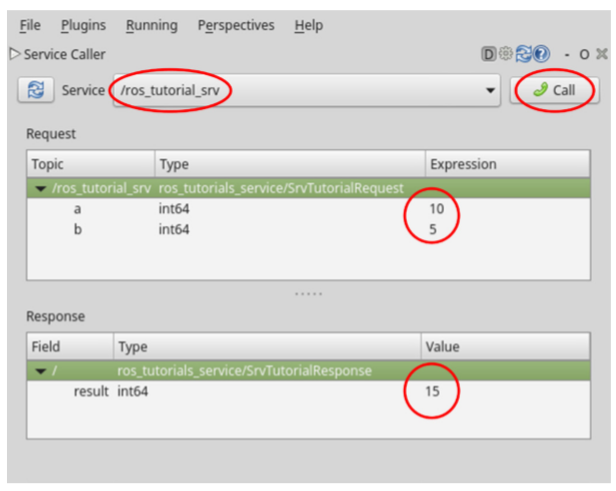
\includegraphics[width=1\linewidth]{src/P.png}
    \centering
    \caption{P} \label{picture:P}
\end{figure}

如果在顶部的“Service”项目中选择服务名称,则会在Request中看到服务请求所 需的信息。要请求服务,请在每个请求信息的Expression中输入信息。我给a输入了10, 给b输入了5。然后点击右上角绿色电话的<Call>图标,服务请求将被执行,屏幕下方的 Response将显示服务响应的结果。 

前面描述的rosservice call具有直接在终端上运行的优点,但对于不熟悉使用Linux 或ROS命令的用户,我们推荐rqt的Service Caller。
\subsection{创建和运行动作服务器和客户端节点}
\subsubsection{生成功能包}
以下命令创建ros_tutorials_action功能包。这个功能包依赖于message_ generation、std_msgs、actionlib_msgs、actionlib和roscpp功能包,因此将这些作 为了依赖选项。
\begin{lstlisting}[frame=single,language=]
    $ cd ~/catkin_ws/src 
    $ catkin_create_pkg ros_tutorials_action message_generation std_msgs actionlib_msgs actionlib roscpp 
\end{lstlisting}
\subsubsection{修改功能包配置文件(package.xml)}
包括修改功能包配置文件(package.xml)的大部分过程与上述话题和服务中描述的 过程非常相似。除了本节的例子中的细节之外,我只会提到源代码并跳过细节。 
\begin{lstlisting}[frame=single,language=xml]
    $ roscd ros_tutorials_action 
    $ gedit package.xml 
\end{lstlisting}

代码如下:
\begin{lstlisting}[frame=single,language=]
    <?xml version="1.0"?> 
    <package>  
    <name>ros_tutorials_action</name>  
    <version>0.1.0</version>  
    <description>ROS tutorial package to learn the action</description>  
    <license>BSD</license>  
    <author>Melonee Wise</author>  
    <maintainer email="pyo@robotis.com">pyo</maintainer>  
    <buildtool_depend>catkin</buildtool_depend>  
    <build_depend>roscpp</build_depend>  
    <build_depend>actionlib</build_depend>  
    <build_depend>message_generation</build_depend>  
    <build_depend>std_msgs</build_depend>  
    <build_depend>actionlib_msgs</build_depend>  
    <run_depend>roscpp</run_depend>  
    <run_depend>actionlib</run_depend>  
    <run_depend>std_msgs</run_depend>  
    <run_depend>actionlib_msgs</run_depend>  
    <run_depend>message_runtime</run_depend>  
    <export></export> 
    </package> 
\end{lstlisting}
\subsubsection{修改构建配置文件(CMakelists.txt)}
与上面介绍的ros_tutorials_topic和ros_tutorials_service节点的构建配置文件不同 的是,如果这些节点的构建过程中生成了msg和srv文件,那么ros_tutorials_action功 能包会生成动作文件(*.action)。此外,还添加了一个新的动作服务器节点和一个动作 客户端节点作为使用它的示例节点。另外,由于我们使用了一个ROS之外的名为Boost的 库,所以多了一个单独的依赖项选项。 
\begin{lstlisting}[frame=single,language=]
    $ gedit CMakeLists.txt 
\end{lstlisting}

代码如下:
\begin{lstlisting}[frame=single,language=]
    cmake_minimum_required(VERSION 2.8.3) 
    project(ros_tutorials_action)
    find_package(catkin REQUIRED COMPONENTS  
        message_generation  
        std_msgs  
        actionlib_msgs  
        actionlib  
        roscpp 
    ) 
    
    find_package(Boost REQUIRED COMPONENTS system) 
    
    add_action_files(FILES Fibonacci.action) 
    generate_messages(DEPENDENCIES actionlib_msgs std_msgs) 
    
    catkin_package(  
        LIBRARIES ros_tutorials_action  
        CATKIN_DEPENDS std_msgs actionlib_msgs actionlib roscpp  
        DEPENDS Boost 
    ) 
    
    include_directories(${catkin_INCLUDE_DIRS} ${Boost_INCLUDE_DIRS}) 
    
    add_executable(action_server src/action_server.cpp) 
    add_dependencies(action_server ${${PROJECT_NAME}_EXPORTED_TARGETS} ${catkin_EXPORTED_TARGETS}) 
    target_link_libraries(action_server ${catkin_LIBRARIES}) 
    
    add_executable(action_client src/action_client.cpp) 
    add_dependencies(action_client ${${PROJECT_NAME}_EXPORTED_TARGETS} ${catkin_EXPORTED_TARGETS}) 
    target_link_libraries(action_client ${catkin_LIBRARIES})
\end{lstlisting}
\subsubsection{创建动作文件}
在CMakeLists.txt文件中加了如下选项。 
\begin{lstlisting}[frame=single,language=]
    add_action_files(FILES Fibonacci.action) 
\end{lstlisting}

这意味着在构建时包含服务Fibonacci.action,这个服务将用于本次的节点中。由于我们目前还没有创建Fibonacci.action,因此我们按以下顺序创建它。
\begin{lstlisting}[frame=single,language=]
    $ roscd ros_tutorials_action → 移动到功能包目录 
    $ mkdir action    → 在功能包中创建一个名为action的动作目录 
    $ cd action     → 移至创建的action目录 
    $ gedit Fibonacci.action   → 创建Fibonacci.action文件并修改内容 
\end{lstlisting}

在动作文件中,三个连字符(---)用作分隔符,第一个是goal消息,第二个是result 消息,第三个是feedback消息。goal消息和result消息之间的关系与上述srv文件相同, 但主要区别在于feedback消息用于指定进程执行过程中的中间值传输。
\begin{lstlisting}[frame=single,language=]
    #goal definition 
    int32 order 
    ---
    #result definition 
    int32[] sequence 
    ---
    #feedback 
    int32[] sequence 
\end{lstlisting}

动作的5种基本消息 除了可以在动作文件中找到的目标(goal)、结果(result)和反馈(feedback) 之外,动作基本上还使用两个额外的消息:取消(cancel)和状态(status)。取消 (cancel)消息使用actionlib\_msgs/GoalID,它在动作运行时可以取消动作客户端和 单独节点上的动作的执行。状态(status)消息可以根据状态转换(如PENDING、 ACTIVE、PREEMPTED和SUCCEEDED)检查当前动作的状态。 
\subsubsection{创建动作服务节点}
在CMakeLists.txt文件中如下添加了生成可执行文件的选项。 
\begin{lstlisting}[frame=single,language=]
    add_executable(action_server src/action_server.cpp)
\end{lstlisting}

也就是说,是通过构建action\_server.cpp文件来创建action\_server可执行文件。我们按以下顺序编写一个执行Action Server节点的功能的程序吧。
\begin{lstlisting}[frame=single,language=]
    $ roscd ros_tutorials_action/src  → 移动到功能包的源代码目录src 
    $ gedit action_server.cpp     → 创建和编辑源代码文件
\end{lstlisting}

代码如下:
\begin{lstlisting}[frame=single,language=]
    #include <ros/ros.h>     // ROS的基本头文件 
    #include <actionlib/server/simple_action_server.h> // 动作库头文件 
    #include <ros_tutorials_action/FibonacciAction.h>  // FibonacciAction动作头文件(生成后自动生成) 
    
    class FibonacciAction 
    { 
        protected:  
        
        // 声明节点句柄  
        ros::NodeHandle nh_;  
        
        // 声明动作服务器  
        actionlib::SimpleActionServer<ros_tutorials_action::FibonacciAction> as_;  
        
        // 用作动作名称  
        std::string action_name_;  
        
        // 声明用于发布的反馈及结果  
        ros_tutorials_action::FibonacciFeedback feedback_;  
        ros_tutorials_action::FibonacciResult result_; 
        
        public:  
        
        // 初始化动作服务器(节点句柄、动作名称、动作后台函数)  
        FibonacciAction(std::string name) :    
            as_(nh_, name, boost::bind(&FibonacciAction::executeCB, this, _1), false),    
            action_name_(name)  
            {    
                as_.start();  
            }  
            ~FibonacciAction(void)  
            {

            }  
        
            // 接收动作目标(goal)消息并执行指定动作(此处为斐波那契数列)的函数。  
            void executeCB(const ros_tutorials_action::FibonacciGoalConstPtr &goal) 
            {    
                ros::Rate r(1);    // 循环周期:1 Hz    
                bool success = true;   // 用作保存动作的成功或失败的变量    
                
                // 斐波那契数列的初始化设置,也添加了反馈的第一个(0)和第二个消息(1)    feedback_.sequence.clear();    
                feedback_.sequence.push_back(0);    
                feedback_.sequence.push_back(1);    
                
                // 将动作名称、目标和斐波那契数列的两个初始值通知给用户    
                ROS_INFO("%s: Executing, creating fibonacci sequence of order %i with seeds %i, %i", action_name_.c_str(), goal->order, feedback_.sequence[0], feedback_.sequence[1]);    
                
                // 动作细节    
                for(int i=1; i<=goal->order; i++)    
                {      
                    // 从动作客户端得知动作取消      
                    if (as_.isPreemptRequested() || !ros::ok())      
                    {        
                        ROS_INFO("%s: Preempted", action_name_.c_str()); // 通知动作取消         
                        as_.setPreempted();     // 取消动作        
                        success = false;     // 看作动作失败并保存到变量        
                        break;      
                    }
                
                    // 除非有动作取消或已达成动作目标      
                    // 将当前斐波纳契数字加上前一个数字的值保存到反馈值。      
                
                    feedback_.sequence.push_back(feedback_.sequence[i] + feedback_.sequence[i-1]);  
                    as_.publishFeedback(feedback_);   // 发布反馈。      
                    r.sleep();      // 按照上面定义的循环周期调用暂歇函数。    
                }    
                
                // 如果达到动作目标值,则将当前斐波那契数列作为结果值传输。    
                if(success)    
                { 
                    result_.sequence = feedback_.sequence;      
                    ROS_INFO("%s: Succeeded", action_name_.c_str());      
                    as_.setSucceeded(result_);    
                }  
            }
    }; 
    
    int main(int argc, char** argv)   // 节点主函数 
    {  
        ros::init(argc, argv, "action_server");  // 初始化节点名称  
        FibonacciAction fibonacci("ros_tutorial_action"); // 声明Fibonacci (动作名: ros_tutorial_action)   
        ros::spin();       // 等待动作目标  
        return 0; 
    }
\end{lstlisting}
\subsubsection{创建客户端节点}
与动作服务器节点一样,客户端节点的设置内容也作为选项加到了CMakeLists.txt文 件中。 
\begin{lstlisting}[frame=single,language=]
    add_executable(action_client src/action_client.cpp) 
\end{lstlisting}

也就是说,通过构建一个名为action_client.cpp的文件来创建action_client可执行文件。我们按照以下顺序编写一个执行动作客户端节点功能的程序。
\begin{lstlisting}[frame=single,language=]
    $ roscd ros_tutorials_action/src  → 移动到功能包的源代码目录src 
    $ gedit action_client.cpp   → 创建并修改源代码文件
\end{lstlisting}

代码如下:
\begin{lstlisting}[frame=single,language=]
    #include <ros/ros.h>     // ROS的基本头文件 
    #include <actionlib/client/simple_action_client.h>  // 动作库头文件 
    #include <actionlib/client/terminal_state.h>   // 动作目标状态头文件 
    #include <ros_tutorials_action/FibonacciAction.h>  // FibonacciAction动作头文件(构建后自动生成) 
    
    int main (int argc, char **argv)    // 节点主函数 
    {  
        ros::init(argc, argv, "action_client");   // 初始化节点名称  
        
        // 声明动作客户端(动作名称:ros_tutorial_action)  actionlib::SimpleActionClient<ros_tutorials_action::FibonacciAction> ac("ros_tutorial_action", true);  

        ROS_INFO("Waiting for action server to start.");  
        ac.waitForServer();      // 等待动作服务器启动  
        
        ROS_INFO("Action server started, sending goal.");  
        ros_tutorials_action::FibonacciGoal goal;   // 声明动作目标  
        goal.order = 20;       // 指定动作目标(进行20次斐波那契运算)  
        ac.sendGoal(goal);     // 发送动作目标  
        
        // 设置动作完成时间限制(这里设置为30秒)  
        bool finished_before_timeout = ac.waitForResult(ros::Duration(30.0));  
        
        // 在动作完成时限内收到动作结果值时  
        if (finished_before_timeout)  
        {    
            // 获取动作目标状态值并将其显示在屏幕上    
            actionlib::SimpleClientGoalState state = ac.getState();    
            ROS_INFO("Action finished: %s",state.toString().c_str());  
        }  
        else
        {
            ROS_INFO("Action did not finish before the time out.");   // 超过了动作完成时限的情况
            //exit
        }
        
        return 0; 
    } 
\end{lstlisting}
\subsubsection{构建节点}
使用以下命令构建ros_tutorials_action功能包的动作文件、动作服务器节点和动 作客户机节点。ros_tutorials_action功能包的源文件位于“~/catkin_ws/src/ros_ tutorials_action/src”目录中,而动作文件位于“~/catkin_ws/src/ros_tutorials_ action/src/action”目录中。 
\begin{lstlisting}[frame=single,language=]
    $ cd ~/catkin_ws && catkin_make    → 转到catkin目录并运行catkin构建
\end{lstlisting}
\subsubsection{运行动作服务器}
我们之前编写的动作服务器在指定动作目标(goal)前不做任何行动,只会等待。因此,执行以下命令时,动作服务器会等待来自动作客户端的目标(goal)指定。运行节点之前不要忘记运行roscore。
\begin{lstlisting}[frame=single,language=]
    $ roscore 
    $ rosrun ros_tutorials_action action_server 
\end{lstlisting}
动作中的动作目标(goal)和结果(result)的用法与服务中的请求和响应类似,这是动作和服务的相似之处。但不同之处在于,动作还有作为中途值的反馈 (feedback)消息。这与服务类似,但其消息的实际通信方式与话题非常类似。因此, 可以通过rqt_graph和rostopic list命令来查看当前动作消息的使用情况。 
\begin{lstlisting}[frame=single,language=]
    $ rostopic list 
    /ros_tutorial_action/cancel 
    /ros_tutorial_action/feedback 
    /ros_tutorial_action/goal 
    /ros_tutorial_action/result 
    /ros_tutorial_action/status 
    /rosout 
    /rosout_agg
\end{lstlisting}

如果想了解更多有关每条消息的信息,请将-v选项添加到rostopic list中。这将单独 显示发布和订阅的话题,如下所示: 
\begin{lstlisting}[frame=single,language=]
    $ rostopic list -v 
    Published topics: 
    * /ros_tutorial_action/feedback [ros_tutorials_action/FibonacciActionFeedback] 1 publisher 
    * /ros_tutorial_action/status [actionlib_msgs/GoalStatusArray] 1 publisher 
    * /rosout [rosgraph_msgs/Log] 1 publisher 
    * /ros_tutorial_action/result [ros_tutorials_action/FibonacciActionResult] 1 publisher 
    * /rosout_agg [rosgraph_msgs/Log] 1 publisher 
    
    Subscribed topics: 
    * /ros_tutorial_action/goal [ros_tutorials_action/FibonacciActionGoal] 1 subscriber 
    * /rosout [rosgraph_msgs/Log] 1 subscriber 
    * /ros_tutorial_action/cancel [actionlib_msgs/GoalID] 1 subscriber
\end{lstlisting}

为了查看可视化信息,请使用以下命令。 动作消息、动作服务器和客户端之间的 关系如图7-8所示,是双向发送和接收。在这里,动作信息由名字ros_tutorial_action/ action_topics统一表示,当关闭菜单中的Actions时,可以看到所有5个消息,如图7-9所 示。在这里我们可以看到,这个动作由5个话题以及发布和订阅这些话题的节点组成。 
\begin{lstlisting}[frame=single,language=]
    $ rqt_graph
\end{lstlisting}
\subsubsection{运行动作客户端}
使用以下命令运行动作客户端。在动作客户端启动的同时,会通过动作目标消息将动作目标设为20。
\begin{lstlisting}[frame=single,language=]
    $ rosrun ros_tutorials_action action_client
\end{lstlisting}

通过设置这个目标值,动作服务器将如下启动斐波那契数列。如果想详细了解中途 值或结果值,可以使用像“rostopic echo /ros_tutorial_action/feedback”这样的 rostopic命令。 
\begin{lstlisting}[frame=single,language=]
    $ rosrun ros_tutorials_action action_server 
    [INFO] [1495764516.294367721]: ros_tutorial_action: Executing, creating fibonacci sequence of order 20 with seeds 0, 1 
    [INFO] [1495764536.294488991]: ros_tutorial_action: Succeeded 
    
    $ rosrun ros_tutorials_action action_client 
    [INFO] [1495764515.999158825]: Waiting for action server to start. 
    [INFO] [1495764516.293575887]: Action server started, sending goal. 
    [INFO] [1495764536.295139830]: Action finished: SUCCEEDED 
    
    $ rostopic echo /ros_tutorial_action/feedback 
    header:   
        seq: 42   
        stamp:     
            secs: 1495764700     
            nsecs: 413836908   
        frame_id: '' 
    status:   
        goal_id:     
            stamp:       
                secs: 1495764698       
                nsecs: 413136891     
            id: /action_client-1-1495764698.413136891   
        status: 1   
        text: This goal has been accepted by the simple action server 
    feedback:   
        sequence: [0, 1, 1, 2, 3]
    ---
\end{lstlisting}
\subsection{参数的用法}
\subsubsection{利用参数创建节点}
修改创建的服务服务器和客户端节点中的service_server.cpp,让通过服务请求输入的a和b不光进行加法运算,还会利用参数让a和b进行四则运算。我们按以下顺序修改service_server.cpp源代码。 
代码如下:
\begin{lstlisting}[frame=single,language=]
    #include "ros/ros.h"      // ROS的基本头文件 
    #include "ros_tutorials_service/SrvTutorial.h"  // SrvTutorial服务头文件 
    
    #define PLUS    1    // 加 
    #define MINUS    2    // 减 
    #define MULTIPLICATION  3    // 乘 
    #define DIVISION    4    // 除 
    
    int g_operator = PLUS; 
    
    // 当有服务请求时,会处理以下内容。 
    // 服务请求设置为req,服务响应设置为res。 
    bool calculation(ros_tutorials_service::SrvTutorial::Request &req,                                     ros_tutorials_service::SrvTutorial::Response &res) 
    {  
        // 根据g_operator参数值进行a和b的运算   
        // 计算后将结果保存到服务响应值中。  
        switch(g_operator)  
        {    
            case PLUS:       res.result = req.a + req.b; break;      
            case MINUS:       res.result = req.a - req.b; break;      
            case MULTIPLICATION:       res.result = req.a * req.b; break;      
            case DIVISION:         
                if(req.b == 0)      
                {        
                    res.result = 0; 
                    break;       
                }       
                else      
                {        
                    res.result = req.a / req.b; 
                    break;       
                }     
            default:res.result = req.a + req.b; break;  
        }   
        
        // 显示服务请求中使用的a和b值,以及相当于服务响应的result值。  
        ROS_INFO("request: x=%ld, y=%ld", (long int)req.a, (long int)req.b); 
        ROS_INFO("sending back response: [%ld]", (long int)res.result);   
        return true; 
    } 
    
    int main(int argc, char **argv)    // 节点主函数 
    { 
        ros::init(argc, argv, "service_server");   // 初始化节点名称 
        ros::NodeHandle nh;      // 声明节点句柄 
        nh.setParam("calculation_method", PLUS);  // 初始化参数 
        
        // 声明服务服务器,创建使用ros_tutorials_service功能包中的SrvTutorial服务文件的  
        // 服务服务器service_server。服务名称是"ros_tutorial_srv" ,  
        // 此服务器当收到服务请求时,会执行一个叫做calculation的函数。 
        ros::ServiceServer ros_tutorial_service_server = nh.advertiseService("ros_tutorial_srv", calculation);  
        ROS_INFO("ready srv server!"); 
        ros::Rate r(10); // 10hz 
        while (1) 
        {   
            // 将运算符改为通过参数收到的值。  
            nh.getParam("calculation_method", g_operator);  
            ros::spinOnce();   // 后台函数处理进程  
            r.sleep();    // 为了反复进入进程而添加的sleep(暂歇)函数 
        }  
        return 0; 
    } 
\end{lstlisting}
\subsubsection{设置参数}
下面的代码是将calculate_method参数设置为PLUS值。 
\begin{lstlisting}[frame=single,language=]
    nh.setParam(“calculation_method”, PLUS);
\end{lstlisting} 

参数可以设置为integers、floats、boolean、string、dictionaries和list 等。
\subsubsection{读取参数}
以下是调取calculation_method参数并设置为g_operator的值的部分代码。因此,g_operator每0.1秒检查一次参数的值,并判断对于通过服务请求收到的值进行何种四则运算。
\begin{lstlisting}[frame=single,language=]
    nh.getParam(“calculation_method”, g_operator); 
\end{lstlisting}
\subsubsection{构建节点和运行节点}
使用以下命令重新构建ros_tutorials_service功能包中的服务服务器节点。 
\begin{lstlisting}[frame=single,language=]
    $ cd ~/catkin_ws && catkin_make
\end{lstlisting}

完成后,使用以下命令运行ros_tutorials_service功能包的service_server节点: 
\begin{lstlisting}[frame=single,language=]
    $ roscore $ rosrun ros_tutorials_service service_server 
    [INFO] [1495767130.149512649]: ready srv server! 
\end{lstlisting}
\subsubsection{查看参数目录}
可以使用“rosparam list”命令查看当前用于ROS网络的参数列表。在显示的列表中,/calculation_method是我们使用的参数。
\begin{lstlisting}[frame=single,language=]
    $ rosparam list 
    /calculation_method 
    /rosdistro 
    /rosversion 
    /run_id 
\end{lstlisting}
\subsubsection{参数的用例}
让我们按照以下命令来设置参数,并观察每次做相同的请求服务但会得到不同的服务 处理。 
\begin{lstlisting}[frame=single,language=]
    $ rosservice call /ros_tutorial_srv 10 5   → 输入要进行四则运算的变量a和b 
    result: 15        → 默认运算加法的结果值 
    $ rosparam set /calculation_method 2    → 减法 
    $ rosservice call /ros_tutorial_srv 10 5 
    result: 5 
    $ rosparam set /calculation_method 3    → 乘法 
    $ rosservice call /ros_tutorial_srv 10 5 
    result: 50 
    $ rosparam set /calculation_method 4    → 除法 
    $ rosservice call /ros_tutorial_srv 10 5 
    result: 2  
\end{lstlisting}

您可以使用“rosparam set”命令更改calculation_method参数。通过更改参数, 您可以看到每次做相同的输入“rosservice call /ros_tutorial_srv 10 5”,却得到不同 的结果值。通过这种方式,ROS中的参数可以改变节点外部的节点的流程、设置和处理。 这是一个非常有用的功能,所以就算现在不使用它,但需要记住。
\subsection{roslaunch的用法}
如果rosrun是执行一个节点的命令,那么roslaunch可以运行多个节点。除此之外, 它还是一种在运行节点时可以附带如下各种选项的ROS命令: 修改参数或节点的名称, 设置节点的命名空间,设置ROS_ROOT及ROS_PACKAGE_PATH,以及环境变量修改等 选项的ROS命令,等。 roslaunch使用“*.launch”文件来设置可执行节点,它基于XML,并提供各个标签 的选项。执行命令是“roslaunch [功能包名称] [roslaunch文件]”。
\subsubsection{roslaunch的应用}
为了解如何使用roslaunch,下面先重命名之前创建的topic_publisher和topic_subscriber节点。只改变名字没有意义,所以让我们运行两个独立的发布者和两个独立的订阅者节点来进行各自的消息通信。

首先,我们编写一个*.launch文件。用于roslaunch的文件具有*.launch文件名,您需要在该功能包目录中创建一个launch 目录,并将launch文件放在该目录中。使用以下命令创建一个目录,并创建一个名为union.launch的新文件。
\begin{lstlisting}[frame=single,language=]
    $ roscd ros_tutorials_topic 
    $ mkdir launch 
    $ cd launch 
    $ gedit union.launch 
\end{lstlisting}

如下编辑union.launch文件的内容。
\begin{lstlisting}[frame=single,language=]
    <launch>    
    <node pkg="ros_tutorials_topic" type="topic_publisher" name="topic_publisher1"/>    
    <node pkg="ros_tutorials_topic" type="topic_subscriber" name="topic_subscriber1"/>    
    <node pkg="ros_tutorials_topic" type="topic_publisher" name="topic_publisher2"/>    
    <node pkg="ros_tutorials_topic" type="topic_subscriber" name="topic_subscriber2"/> 
    </launch> 
\end{lstlisting}

在<launch>标签中,描述了使用roslaunch命令运行节点所需的标签。<node>描述 了roslaunch运行的节点。选项包括pkg、type和name。 

pkg   功能包的名称

type  实际运行的节点的名称(节点名)

name   与上述type对应的节点被运行时,起的名称(运行名)。一般情况下使用与type相同的名称,但可以根据需要,在运行时更改名称。 

如果创建了roslaunch文件,可以如下运行union.launch。请注意,当用roslaunch命令运行多个节点时,运行中的节点的输出(info、error等)不会显示在终端屏幕上, 这会使调试变得困难。如果此时添加了--screen选项,终端上运行的所有节点的输出将显示在终端屏幕上。 
\begin{lstlisting}[frame=single,language=]
    $ roslaunch ros_tutorials_topic union.launch --screen
\end{lstlisting}

运行结果会如何? 首先,让我们使用以下命令看看当前正在运行的节点吧。 
\begin{lstlisting}[frame=single,language=]
    $ rosnode list 
    /rosout 
    /topic_publisher1 
    /topic_publisher2 
    /topic_subscriber1 
    /topic_subscriber2
\end{lstlisting}

可以看到,topic_publisher节点已被重命名为topic_publisher1和topic_publisher2,而topic_subscriber节点已被重命名为topic_subscriber1和topic_ subscriber2。这四个节点均在运行中。
\begin{figure}[htbp]
    \centering
    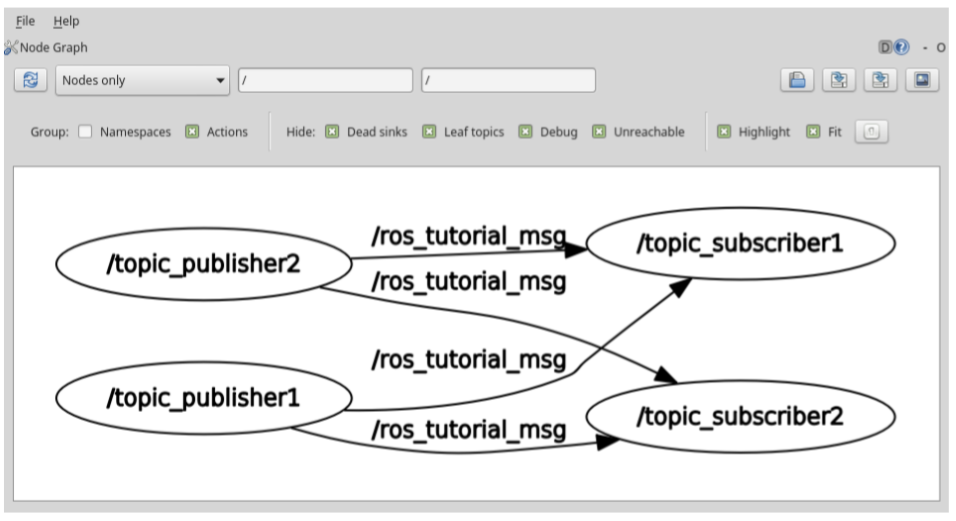
\includegraphics[width=1\linewidth]{src/Q.png}
    \centering
    \caption{Q} \label{picture:Q}
\end{figure}

问题在于,我们通过rqt_graph看到,与“两个发布者节点和两个订阅者 节点中的每一个发布者和订阅者都只与一个订阅者和发布者进行单独的通信”的当初的 目的不符,两个订阅者都在订阅两个发布者的消息。这是因为我们只是改变了节点的名 字,而没有改变要使用的消息的名字。我们用另一个roslaunch命名空间标记来解决这个问题。让我们修改之前创建的union.launch文件,如下所示。
\begin{lstlisting}[frame=single,language=]
    $ roscd ros_tutorials_topic/launch 
    $ gedit union.launch 
\end{lstlisting}

\begin{lstlisting}[frame=single,language=]
    <launch>  
    <group ns="ns1">    
    <node pkg="ros_tutorials_topic" type="topic_publisher" name="topic_publisher"/>    
    <node pkg="ros_tutorials_topic" type="topic_subscriber" name="topic_subscriber"/>  
    </group>  
    <group ns="ns2">    
    <node pkg="ros_tutorials_topic" type="topic_publisher" name="topic_publisher"/>    
    <node pkg="ros_tutorials_topic" type="topic_subscriber" name="topic_subscriber"/>  
    </group> 
    </launch> 
\end{lstlisting}

<group>是对指定节点进行分组的标签。选项有ns。这是命名空间(name space),是组的名称,属于该组的节点和消息都包含在由ns指定的名称中。

再一次,我们来检查rqt_graph节点之间的连接和消息发送/接收状态。这一次,如图所示,我们可以看到,我们实现了我们最初的目的。
\begin{figure}[htbp]
    \centering
    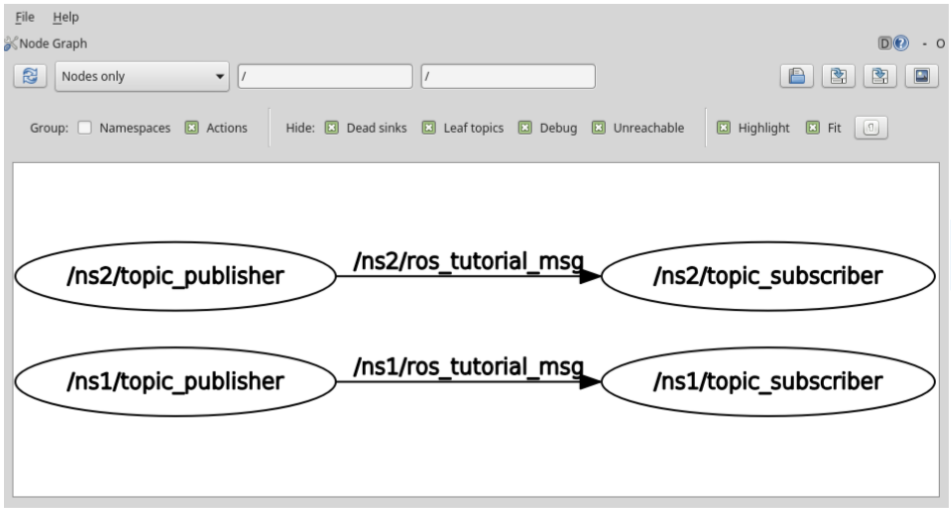
\includegraphics[width=1\linewidth]{src/R.png}
    \centering
    \caption{R} \label{picture:R}
\end{figure}
\subsubsection{Launch标签}
在launch文件中根据XML的编写方式可以实现多种功能。launch中使用的标签如下所示。

<launch> 指roslaunch语句的开始和结束。

<node>  这是对于节点运行的标签。您可以更改功能包、节点名称和执行名称。

<machine>  可以设置运行该节点的PC的名称、address、ros-root和ros-package-path。

<include>   您可以加载属于同一个功能包或不同的功能包的另一个launch,并将其作为一个launch 文件来运行。

<remap>  可以更改节点名称、话题名称等等,在节点中用到的ROS变量的名称。

<env>  设置环境变量,如路径和IP(很少使用)。

<param>  设置参数名称、类型、值等

<rosparam>  可以像rosparam命令一样,查看和修改load、dump和delete等参数信息。

<group>  用于分组正在运行的节点。

<test>  用于测试节点。类似于<node>,但是有可以用于测试的选项。

<arg>  可以在launch文件中定义一个变量,以便在像下面这样运行时更改参数。

如下面的例子所示,利用其中的参数设置<param>和launch文件中的变量<arg>,可以在运行launch时从外部修改内部变量,因此甚至可以在运行的同时修改节点内部的参数。这是一个非常有用和广泛使用的方法,因此需要掌握。

\begin{lstlisting}[frame=single,language=]
    <launch>   
    <arg name="update_period" default="10" />  
    <param name="timing" value="$(arg update_period)"/> 
    </launch> 
\end{lstlisting}

\begin{lstlisting}[frame=single,language=]
    $ roslaunch my_package my_package.launch update_period:=30
\end{lstlisting}
\section{机器人、传感器和电机}
机器人主要分为硬件和软件。机械、电机、齿轮、电路和传感器被归类为硬件。直接驱动或控制机器人硬件的微控制器级别的固件,以及利用从传感器获得的信息进行识别、制图、导航和动作规划的应用软件均被分类为软件。ROS属于应用软件的范畴,根据功能,ROS的功能包被分类为机器人功能包、专为传感器的传感器功能包和专为驱动部的电机功能包。公共机器人功能包可以在http://robots.ros.org/ 找到。
\subsection{机器人功能包}
\subsection{传感器功能包}
\subsubsection{传感器的类型}
\subsubsection{传感器功能包的分类}
\subsection{相机}
\subsubsection{USB摄像头相关功能包}
\subsubsection{USB摄像头测试}
\subsubsection{查看图像信息}
\subsubsection{远程传输图像}
\subsubsection{相机校准}
\subsection{深度相机(Depth Camera)}
\subsubsection{Depth Camera的类型}
\subsubsection{Depth Camera测试}
\subsubsection{Point Cloud Data(点云数据)的可视化}
\subsubsection{Point Cloud Data相关库}
\subsection{激光距离传感器}
\subsubsection{LDS传感器距离测量原理}
\subsubsection{LDS测试}
\subsubsection{可视化LDS的距离值}
\subsubsection{LDS的应用}
\subsection{电机功能包}
\subsubsection{Dynamixel舵机}
\subsection{已公开的功能包的用法}
\subsubsection{搜索功能包}
\subsubsection{安装依赖包}
\subsubsection{安装功能包}
\subsubsection{运行功能包}
\section{嵌入式系统}
\subsection{OpenCR}
\subsubsection{特点}
\subsubsection{控制板规格}
\subsubsection{搭建开发环境}
\subsubsection{OpenCR例程}
\subsection{RosseriaL}
\subsubsection{Rosserial server}
\subsubsection{Rosserial client}
\subsubsection{Rosserial协议}
\subsubsection{Rosserial的约束条件}
\subsubsection{安装rosserial}
\subsubsection{Rosserial例程}
\subsection{TurtleBot3的固件}
\subsubsection{TurtleBot3 Burgeri固件}
\subsubsection{TurtleBot3 Waffle和Waffle Pi固件}
\subsubsection{Turtlebot3配置固件}
\section{移动机器人}
\subsection{ROS支持的机器人}
\subsection{TurtleBot3系列机器人}
\subsection{TurleBot3的硬件}
\subsection{Turtlebot3软件}
\subsection{Turtlebot3的开发环境}
\subsection{Turtlebot3远程控制}
\subsubsection{遥控TurtleBot3}
\subsubsection{可视化TurtleBot3}
\subsection{Turtlebot3话题}
\subsubsection{订阅话题}
\subsubsection{通过订阅话题控制机器人}
\subsubsection{发布话题}
\subsubsection{通过发布话题识别机器人状态}
\subsection{使用RViz仿真Turtlebot3}
\subsubsection{仿真}
\subsubsection{运行虚拟机器人}
\subsubsection{Odometry和TF}
\subsection{利用Gazebo仿真Turtlebot3}
\subsubsection{Gazebo仿真器}
\subsubsection{启动虚拟机器人}
\subsubsection{虚拟SLAM和导航}
\section{SLAM和导航}
\subsection{导航及其组成要素}
\subsubsection{移动机器人的导航}
\subsubsection{地图}
\subsubsection{测量或估计机器人姿态的功能}
\subsubsection{识别障碍物如墙壁和物体}
\subsubsection{计算最优路径和行驶功能}
\subsection{SLAM实习篇}
\subsubsection{对于使用SLAM的机器人的硬件限制}
\subsubsection{SLAM的实验环境}
\subsubsection{用于SLAM的ROS功能包}
\subsubsection{运行SLAM}
\subsection{利用预先准备好的bag文件运行的SLAM}
\subsection{SLAM应用篇}
\subsubsection{地图}
\subsubsection{SLAM所需的信息}
\subsubsection{SLAM的处理过程}
\subsubsection{坐标变换(TF)}
\subsubsection{Turtlebot3\_slam功能包}
\subsection{SLAM理论篇}
\subsubsection{SLAM}
\subsubsection{多种位置估计(localization)方法论}
\subsection{导航实战篇}
\subsubsection{用于导航的ROS功能包}
\subsubsection{运行导航}
\subsection{导航应用程序}
\subsubsection{导航}
\subsubsection{导航所需的信息}
\subsubsection{Turtlebot3\_navigation的各节点和话题状态}
\subsubsection{Turtlebot3\_navigation设置}
\subsubsection{设置turtlebot3\_navigation的详细参数}
\subsection{导航理论篇}
\subsubsection{Costmap}
\subsubsection{AMCL}
\subsection{Dynamic Window Approach(DWA)}
\section{服务机器人}
\subsection{配关服务机器人}
\subsection{关服务机器人的结构}
\subsubsection{系统结构}
\subsubsection{系统设计}
\subsubsection{服务核心节点}
\subsubsection{服务主节点}
\subsubsection{服务从节点}
\subsection{用ROS Java进行Android平板PC编程}
\section{机械手臂}
\subsection{机械手臂介绍}
\subsubsection{机械手臂的结构和控制}
\subsubsection{机械手臂和ROS}
\subsection{OpenManipulator。建模和仿真}
\subsubsection{OpenManipulator}
\subsubsection{机械手臂建模}
\subsubsection{Gazebo设置}
\subsection{MoveIt!}
\subsubsection{Move\_group}
\subsubsection{MoveIt!Setup Assistant}
\subsubsection{Gazebo仿真}
\subsection{应用于实际平台}
\subsubsection{准备和控制OpenManipulator}
\subsubsection{OpenManipulator与turtleBot3Waffle及Waffle Pi}
\end{document}